% Copyright (C) 2014-2020 by Thomas Auzinger <thomas@auzinger.name>

\documentclass[draft,final]{vutinfth} % Remove option 'final' to obtain debug information.

% Load packages to allow in- and output of non-ASCII characters.
\usepackage{lmodern}        % Use an extension of the original Computer Modern font to minimize the use of bitmapped letters.
\usepackage[T1]{fontenc}    % Determines font encoding of the output. Font packages have to be included before this line.
\usepackage[utf8]{inputenc} % Determines encoding of the input. All input files have to use UTF8 encoding.

% Extended LaTeX functionality is enables by including packages with \usepackage{...}.
\usepackage{amsmath}    % Extended typesetting of mathematical expression.
\usepackage{amssymb}    % Provides a multitude of mathematical symbols.
\usepackage{mathtools}  % Further extensions of mathematical typesetting.
\usepackage{microtype}  % Small-scale typographic enhancements.
\usepackage[inline]{enumitem} % User control over the layout of lists (itemize, enumerate, description).
\usepackage{multirow}   % Allows table elements to span several rows.
\usepackage{booktabs}   % Improves the typesettings of tables.
\usepackage{subcaption} % Allows the use of subfigures and enables their referencing.
\usepackage[ruled,linesnumbered,algochapter]{algorithm2e} % Enables the writing of pseudo code.
\usepackage[usenames,dvipsnames,table]{xcolor} % Allows the definition and use of colors. This package has to be included before tikz.
\usepackage{nag}       % Issues warnings when best practices in writing LaTeX documents are violated.
\usepackage{hyperref}  % Enables cross linking in the electronic document version. This package has to be included second to last.
\usepackage[acronym,toc]{glossaries} % Enables the generation of glossaries and lists fo acronyms. This package has to be included last.
\usepackage[round]{natbib}
\usepackage{amsfonts}
\usepackage{multibib}
\usepackage{bm}
\usepackage{usebib}
\bibinput{core}

\definecolor{tab:green}{RGB}{0,128,0}
\definecolor{tab:red}{RGB}{214,39,32}
\definecolor{tab:orange}{RGB}{255,127,0}
\definecolor{tab:blue}{RGB}{31,119,176}
\definecolor{tab:purple}{RGB}{148,103,176}

\usepackage{soul}
\usepackage[outline]{contour}
\DeclareRobustCommand{\colorindicator}[2]{ {%
\begingroup%
\setul{0.25ex}{0.4ex}%
\contourlength{0.2ex}%
\setulcolor{#1}%
\ul{{\phantom{#2}}}\llap{\contour{white}{#2}} %
%  \ul{{\phantom{#2}}}\llap{\contour{white}{#2}} \textcolor{#1}{\tiny{$\blacksquare$}}%
\endgroup%
}}

\newcites{Online}{Non-Scientific Bibliography}

% Define convenience functions to use the author name and the thesis title in the PDF document properties.
\newcommand{\authorname}{Rafael Sterzinger} % The author name without titles.
\newcommand{\thesistitle}{Weighting Extrinsic and Intrinsic Rewards in Reinforcement Learning}
%Prediction Error based Curiosity and How to Combine Extrinsic and Intrinsic Rewards
\newcommand{\thesissubtitle}{}% The title of the thesis. The English version should be used, if it exists.
\newcommand{\p}[1]{see p. #1}

% Set PDF document properties
\hypersetup{
pdfpagelayout   = TwoPageRight,           % How the document is shown in PDF viewers (optional).
linkbordercolor = {Melon},                % The color of the borders of boxes around crosslinks (optional).
pdfauthor       = {\authorname},          % The author's name in the document properties (optional).
pdftitle        = {\thesistitle},         % The document's title in the document properties (optional).
pdfsubject      = {Bachelor's thesis on \thesistitle; Written by \authorname in the context of TARO/INSO research group},         % The document's subject in the document properties (optional).
pdfkeywords     = {deep reinforcement learning, sparse rewarding environments, prediction-error based curiosity, balancing extrinsic and intrinsic rewards} % The document's keywords in the document properties (optional).
}

\setpnumwidth{2.5em}        % Avoid overfull hboxes in the table of contents (see memoir manual).
\setsecnumdepth{subsection} % Enumerate subsections.

\nonzeroparskip             % Create space between paragraphs (optional).
\setlength{\parindent}{0pt} % Remove paragraph identation (optional).

\makeindex      % Use an optional index.
\makeglossaries % Use an optional glossary.
%\glstocfalse   % Remove the glossaries from the table of contents.

% Set persons with 4 arguments:
%  {title before name}{name}{title after name}{gender}
%  where both titles are optional (i.e. can be given as empty brackets {}).
\setauthor{}{\authorname}{}{male}
\setauthorextra
\setadvisor{Ao.Univ.Prof. Dipl.-Ing. Dr.techn.}{Thomas Grechenig}{}{male}

% For bachelor and master theses:
\setfirstassistant{Dipl.-Ing.}{Michael Ressmann}{}{male}

% For dissertations:
%\setfirstreviewer{Pretitle}{Forename Surname}{Posttitle}{male}
%\setsecondreviewer{Pretitle}{Forename Surname}{Posttitle}{male}

% For dissertations at the PhD School and optionally for dissertations:
%\setsecondadvisor{Pretitle}{Forename Surname}{Posttitle}{male} % Comment to remove.

% Required data.
\setregnumber{11778282}
\setdate{10}{08}{2020} % Set date with 3 arguments: {day}{month}{year}.
\settitle{\thesistitle}{\thesistitle} % Sets English and German version of the title (both can be English or German). If your title contains commas, enclose it with additional curvy brackets (i.e., {{your title}}) or define it as a macro as done with \thesistitle.
\setsubtitle{\thesissubtitle}{\thesissubtitle} % Sets English and German version of the subtitle (both can be English or German).

% Select the thesis type: bachelor / master / doctor / phd-school.
% Bachelor:
\setthesis{bachelor}
%
% Master:
%\setthesis{master}
%\setmasterdegree{dipl.} % dipl. / rer.nat. / rer.soc.oec. / master
%
% Doctor:
%\setthesis{doctor}
%\setdoctordegree{rer.soc.oec.}% rer.nat. / techn. / rer.soc.oec.
%
% Doctor at the PhD School
%\setthesis{phd-school} % Deactivate non-English title pages (see below)

% For bachelor and master:
\setcurriculum{Business Informatics }{Wirtschaftsinformatik} % Sets the English and German name of the curriculum.

% For dissertations at the PhD School:
%\setfirstreviewerdata{Affiliation, Country}
%\setsecondreviewerdata{Affiliation, Country}


\newacronym{im}{IM}{Intrinsic Motivation}
\newacronym{em}{EM}{Extrinsic Motivation}
\newacronym{rl}{RL}{Reinforcement Learning}
\newacronym{mdp}{MDP}{Markov Decision Process}
\newacronym{ml}{ML}{Machine Learning}
\newacronym{mlp}{MLP}{Multi-Layer Perceptron}
\newacronym{nn}{NN}{Neural Network}
\newacronym{dp}{DP}{Dynamic Programming}
\newacronym{dl}{DL}{Deep Learning}
\newacronym{drl}{DRL}{Deep Reinforcement Learning}
\newacronym{mc}{MC}{Monte-Carlo}
\newacronym{td}{TD}{Temporal-Difference}
\newacronym{ppo}{PPO}{Proximal Policy Optimization}
\newacronym{trpo}{TRPO}{Trust Region Policy Optimization}
\newacronym{relu}{ReLU}{Rectified Linear Unit}
\newacronym{rf}{RF}{Random Features}
\newacronym{idf}{IDF}{Inverse Dynamics Features}
\newacronym{cnn}{CNN}{Convolutional Neural Networks}
\newacronym{vae}{VAE}{Variational Auto-Encoders}
\newacronym{icm}{ICM}{Intrinsic Curiosity Module}

\begin{document}

    \frontmatter % Switches to roman numbering.
%  The structure of the thesis has to conform to the guidelines at
%  https://informatics.tuwien.ac.at/study-services

    \addtitlepage{naustrian} % German title page (not for dissertations at the PhD School).
    \addtitlepage{english} % English title page.
    \addinsotitlepage{naustrian}
    \addstatementpage

    \begin{danksagung*}

        %    Ich möchte diese Arbeit meine beiden Eltern widmen, welche mich während meines Studiums nicht nur finanzielle, sondern auch moralisch unterstützt haben. Insbesondere während der Verfassung dieser %Bachelorarbeit möchte ich mich dafür bedanken, dass ihr immer für mich da wart und mich in meinem Bestreben ermutigt habt.

        %    Ebenfalls ein großes Dankeschön möchte ich an meinen Betreuer Michael Ressmann ausprechen, welcher mir während der Planung und Durchführung der Arbeit den nötigen Freiraum gegeben hat, zeitgleich aber auch %darauf geachtet hat, dass ich mich in meinem Vorhaben nicht übernehme. Außerdem möchte ich mich bei ihm für sein gutes Feedback sowie für die rasche Benotung meiner Bachelorarbeit bedanken, welcher aufgrund %zeitlicher Beschränkungen meinerseits notwendig war.

        %    Außerdem möchte ich mich bei meinen Freunden bedanken, insbesondere bei meinen langjährigen Freunden, Stefan Zeller und Vinzenz Schicho, welche mich in diesen intensiven Wochen begleitet und mir gut zugesprochen haben.

        %Zu guter Letzt
% wöchentlichen treffen um energie zu tanken für weiteres verfassen
%TODO danke für korrektur lesen
    \end{danksagung*}

    \begin{acknowledgements*}
        % I would like to dedicate this work to my parents, who supported me not only financially but also morally during my studies. In particular while writing this Bachelor's thesis, I would like to thank both of you% for always being there for me and for encouraging me in my endeavors.

        % I would also like to express a big thank you to my supervisor Michael Ressmann, who gave me the necessary freedom during the planning and execution of this Bachelor's thesis, but at the same time also made %sure that I did not take on too much during my project. I would also like to thank him for his good feedback and for the quick grading of my thesis, which was necessary due to time constraints on my part.

        % Also, I would like to thank my friends, especially by my long-standing friends, Stefan Zeller and Vinzenz Schicho, who accompanied me during these intensive weeks and cheered me up.
        % Last but not least,
%TODO danke für korrektur lesen

    \end{acknowledgements*}

    \begin{kurzfassung}
    \end{kurzfassung}

    \begin{abstract}
    \end{abstract}

% Select the language of the thesis, e.g., english or naustrian.
    \selectlanguage{english}

% Add a table of contents (toc).
    \tableofcontents % Starred version, i.e., \tableofcontents*, removes the self-entry.

% Switch to arabic numbering and start the enumeration of chapters in the table of content.
    \mainmatter


    \chapter{Introduction}

    %TODO write introduction


    \section{Problem Description}\label{sec:problem-description}
    In \gls{rl}, algorithms mainly depend on carefully designed extrinsic reward functions which are comparable with feedback to an agent's behaviour.
    In order to teach an agent a certain desired behaviour, it has to optimize this reward function by trial and error.
    This traditional approach yielded multiple astonishing results over the last decade.
    Tasks which award rewards densely, i.e.\ almost after every performed action, are common for these results.
    In opposite to dense rewards, sparse rewards are scattered in the environment which poses the problem that they occur too rarely for an agent to pick up the needed skills.
    An example for environments with sparse rewards are tasks which depend heavily on exploration, e.g. \textit{Montezumas's revenge}.
    \\\\
    An approach to tackle these problems is curiosity, an organism's \gls{im} to spontaneously explore its environment.
    \gls{im} allows an agent to incrementally learn valuable skills independently of its given task by an intrinsic and therefore a more general reward function.
    In general, the concept of intrinsic and extrinsic evolves around the question of why an agent performed a certain action in a given state.
    Since \gls{im} became an important part of \gls{rl}, the following challenges were crystallized out by~\cite[\p{6}]{aubret_survey_2019}:

    \begin{itemize}
        \item \textbf{Sparse rewards:} The agent never reaches a reward signal in case of sparse rewards.
        \item \textbf{State representation:} The agent does not manage to learn a representation of its observations with independent features or meaningful distance metrics.
        \item \textbf{Building option:} The agent is unable to learn abstract high-level decisions independently from the task.
        \item \textbf{Learning a curriculum:} The agent hardly defines a curriculum among its available goals without expert knowledge.
        \label{enm:challenges}
    \end{itemize}

    Besides a general introduction to \gls{im} and its challenges in \gls{rl} (see chapter~\ref{ch:intrinsic-motivation-in-reinforcement-learning}), this Bachelor's thesis has its focus on knowledge acquisition through exploration.
    Knowledge acquisition is described as the agent's motivation to find new knowledge about its environment, meaning that it is interested in things it can or cannot control, the function of the world, discovering new areas, or understanding the proximity.
    Concerning exploration, one approach is error prediction which is the agent's difficulty to predict the state following a state-action tuple.
    This idea is heavily explored by~\cite{burda_large-scale_2018-1} and its prior work of~\cite{pathak_curiosity-driven_2017-1}, both of which are core references of this thesis.
    \\\\
    Building upon the findings of~\citeauthor{burda_large-scale_2018-1}, this Bachelor's thesis eyes on answering the question on how to optimally combine intrinsic and extrinsic rewards in order to maximize an agents score, primarily in sparse but also in dense environments.
    Furthermore, it will evaluate if a balanced reward combination tackles the noisy-TV problem, proposed by~\cite{schmidhuber_formal_2010}.
    The noisy-TV problem, also known as the white-noise problem, is an algorithm's inability to handle the local stochasticity of the environment: "\textit{\ldots random noise in a 3D environment attracts the agent; it will passively watch the noise since it will not be able to predict the next state.}"\cite[\p{10}]{aubret_survey_2019}
    \\\\
    The domain of the given problem description is \gls{rl} with a focus on the model of knowledge acquisition via exploration.


    \section{Expected Results}\label{sec:expected-results}
    As aforementioned, the goal pursued by this Bachelor's thesis is to build upon the results of~\citeauthor{burda_large-scale_2018-1} and to pursue their posed question on how to optimally combine intrinsic ($r_{int}$) and extrinsic ($r_{ext}$) rewards.
    In order to do so, the coefficients $\alpha$ and $\beta$ have to be selected accordingly.
    \[r=\alpha r_{int} + \beta r_{ext}\]
    From that, an optimal solution to this equation maximizes the agent's overall reward when testing.
    \\\\
    After a re-implementation of the proposed algorithms, the benchmarks are expected to at least match the mean rewards mentioned in the \textit{Additional Results} section from the underlying paper.
    In this section, the authors explored the performance of combined rewards on five different Atari games and already showed that the combination of rewards yield a higher mean reward and thus an exhaustive hyperparameter tuning should certainly improve these results.
    However, this poses the question of how algorithms with combined rewards perform in densely rewarding environments as well.
    Therefore, it would be interesting to observe the performance in environments with dense rewards too since if there might be an improvement to see as well.
    \\\\
    In the \textit{Discussion} section,~\citeauthor{burda_large-scale_2018-1} mention the limitations of prediction-error based curiosity which was earlier introduced with the so-called noisy-TV problem.
    Given this problem, the question is raised on whether or not it is possible to tackle the agent's distraction through curiosity with \gls{em}.
    This question will be pursued during the evaluation process with the posed hypothesized that it is possible to overcome an agent's distraction and the assumption that \gls{em} has a higher impact on the distraction in a densely rewarding environment than in a sparse one.
    \\\\
    With the given prospect to beat state-of-the-art approaches to environments with sparse rewards and evaluate the amount of extrinsic reward needed to put a distracted agent back on track, it is the opportunity to pursue important constructs, which reflect the natural human propensity to learn and assimilate, in the domain of computer science that motivated this Bachelor's thesis.


    \section{Methodological Approach}\label{sec:methodological-approach}
    In order to answer the question on how to optimally combine intrinsic and extrinsic rewards, the thesis builds upon the released source code and environments from~\cite{burda_large-scale_2018-1} and~\cite{pathak_curiosity-driven_2017-1} which can be observed on these websites. \footnote{\url{https://pathak22.github.io/large-scale-curiosity}}\footnote{\url{https://pathak22.github.io/noreward-rl/}}
    Therefore, this Bachelor's thesis follows a programming approach which relies on the same tools used by the preceding authors, since it guarantees optimal reproducibility of their results.
    In an overview, these tools are the \index{Python}\textit{Python}\footnote{\url{https://www.python.org/}} programming language, the \gls{ml} platform \index{TensorFlow}\textit{TensorFlow}\footnote{\url{https://www.tensorflow.org/}}, and lastly the \index{OpenAI Gym}\textit{OpenAI Gym}\footnote{\url{https://gym.openai.com/}} which is a toolkit for developing and comparing \gls{rl} algorithms.
    \\\\
    The development progress is structured into the following five milestones:

    \begin{enumerate}
        \item Setting-up of the environment, including the installation of the \index{CUDA}\textit{CUDA}\footnote{\url{https://developer.nvidia.com/cuda-toolkit}} toolkit and the \index{cuDNN}\textit{cuDNN}\footnote{\url{https://developer.nvidia.com/cudnn}]} library
        \item Implementing a Proximal Policy Optimization (PPO) algorithm according to~\cite{schulman_proximal_2017}, using extrinsic rewards
        \item Adding an Intrinsic Curiosity Module, published by~\cite{pathak_curiosity-driven_2017-1}, in order to allow for intrinsic rewards
        \item Tuning of the coefficients $\alpha,\beta$ and comparison to state-of-the-art approaches
        \item Recreation of the synthetic generated noisy-TV problem, proposed by~\cite{burda_large-scale_2018-1}
    \end{enumerate}

    During this incremental process, an emphasis is laid on two out of five sparse Atari 2600 games which were categorized by~\cite{bellemare_unifying_2016} and picked by~\citeauthor{burda_large-scale_2018-1}, namely \textit{Montezumas's revenge} and \textit{Freeway}.
    \\\\
    Regarding milestone three, \textit{Random Features} and \textit{Inverse Dynamics Features} as introduced by~\citeauthor{burda_large-scale_2018-1} are primarily the focus.
    Concerning milestone four and the comparison to state-of-the-art approaches, chapter~\ref{sec:state_of_the_art} of this thesis allows for a current in-depth overview of methods based on knowledge acquisition via exploration.
    Additionally to the aforementioned practical part, the theoretical aspect of this Bachelor's thesis will be covered by exhaustive literature research with an emphasize on directly comparable approaches, i.e.\ prediction-error based curiosity~\citep{burda_large-scale_2018-1}.


    \section{Thesis Outline}\label{sec:thesis-outline}


    \glsresetall


    \chapter{Reinforcement Learning Background}\label{ch:reinforcement-learning-background}

    %TODO write introduction


    \section{Reinforcement Learning Problem}\label{sec:reinforcement-learning-problem}
    Reinforcement Learning, the science of decision making, is about learning the consequences of performed actions and using this knowledge to maximize a numeric \textit{reward signal} which should direct the search for a given objective~\citep[\p{1f}]{sutton_reinforcement_2018}.
    \gls{rl} problems are tackled by a learner or rather an \textit{agent} that performs actions in an \textit{environment} in a trial and error paradigm.
    The agent has no prior knowledge of the consequences of the possible actions but has to explore which action to take in a certain situation to maximize the number of obtainable rewards.
    An additional difficulty is added if the reward for an action is delayed because the agent has to understand which of the executed actions led to the desirable reward it received far ahead in the future.
    Lastly, a proper weighting between exploration and exploitation has to be developed as the agent must exploit actions with known consequences to perform well but also explore new ones in order to improve~\citep{kaelbling_reinforcement_1996}.

    In addition to the aforementioned environment, agent, and reward signal, \gls{rl} consists of further subelements since it would be desirable e.g. not only to know the immediate reward but also to gain measurement for all possible future rewards from a given state onward.
    For this purpose, a \textit{value function} is used.
    It acts as a long-term indicator that describes the attractiveness of a state an agent might result in after interacting with its environment.
    This measurement is interesting because there could be an action which leads to a high immediate reward but results in an undesirable state with no future rewards.
    Furthermore, the agent should pick up a \textit{policy} that consists of state-action tuples which should be refined and adjusted depending on the received rewards.
    Lastly, the agent may want to build a \textit{model} which estimates the environment's behaviour, in order to plan its actions.
    This final addition divides the \gls{rl} problem spectrum into two parts: model-free and model-based approaches~\citep[6f]{sutton_reinforcement_2018}.


    In opposite to other known \gls{ml} disciplines such as \textit{supervised learning}, there is no supervisor in \gls{rl} that explicitly tells the agent which action would be correct in a given state and because of that, the agent has to come up with its policy based on the repeated feedback it receives from the immediate reward and the following state~\citep{kaelbling_reinforcement_1996}.
    This spares the necessity of creating a training dataset with corresponding state-action tuples beforehand and thus \gls{rl} is the preferred choice in cases where an agent interacts with and influences its environment.
    Furthermore, teaching based on supervision would also mean that an agent will be limited to the labelling ability of its supervisor which is another reason why it must be able to learn from its own experiences~\citepOnline{silver_lecture_2015-2}.
    Since \gls{rl} is quite distinct from supervised learning and does not rely on labelled examples, it is sometimes misclassified as \textit{unsupervised learning} which has the purpose to find structure in unlabelled data.
    However, this is not applicable for \gls{rl} as the agent has to maximize a reward function and not to find structure in data.
    Therefore, \citet[\p{2}]{sutton_reinforcement_2018} classified \gls{rl} as the third subfield of \gls{ml}.


    \section{Markov Decision Processes}\label{sec:markov-decision-processes}
    In order to formalize the \gls{rl} problem, the idea and notation of an \gls{mdp} is used to notate the sequential interactions between an agent and its environment.
    At every discrete time-step, $t = 0,1,2,3, \ldots \in \mathbb{N}$, the agent observes the current state, $S_t \in \mathit{S}$, of the environment and selects an available action in a given state, $A_t \in \mathit{A}(s)$.
    Sometimes this notation is simplified to $A_t \in \mathit{A}$ assuming that the action set $\mathit{A}$ does not depend on the state~\citep[\p{48}]{sutton_reinforcement_2018}.
    Once the agent has selected an action, it obtains a scalar reward $R_{t+1} \in \mathit{R} \subset \mathbb{R}$ and depending on the action, the environment transforms into a subsequent state $S_{t+1}$~\eqref{fig:rl_problem}.
    By means of continuous interactions between the agent and the environment, a trajectory of the form $S_0,A_0,R_1,S_1,A_1,R_2,S_2,A_2,R_3,\ldots$ is created.

    \begin{figure}[h]
        \centering
        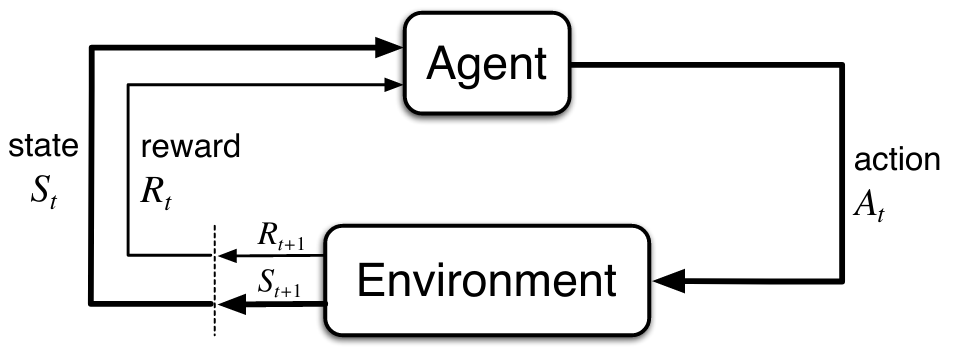
\includegraphics[width=\textwidth]{figures/rl_problem.png}
        \caption[The \gls{rl} framework formalized as an \gls{mdp}]{The \gls{rl} framework formalized as an \gls{mdp}\protect\footnotemark}
        \label{fig:rl_problem}
    \end{figure}

    \footnotetext{\cite[\p{48}]{sutton_reinforcement_2018}}

    In a finite horizon, the agent has to plan only a fixed number of time-steps ahead and the sets $\mathit{S},\mathit{A}\text{, and }\mathit{R}$ are limited~\citep[\p{47f}]{sutton_reinforcement_2018,kaelbling_reinforcement_1996}.
    Furthermore, the possibility that the values $s'\in \mathit{S}$ and $r \in \mathit{R}$ may occur at a time-step $t+1$, can be described with a probability~\eqref{eq:distribution} solely depending on the action $a \in \mathit{A}(s)$ taken in a preceding state $s \in \mathit{S}$.

    \begin{equation}
        p(s',r|s,a) = P\{S_{t+1}=s', R_{t+1}=r | S_t=s, A_t=a\}\label{eq:distribution}
    \end{equation}

    Since $p$ describes a probability, the sum over all possible combinations of $s$ and $a$ must be equal to 1.
    Moreover, the individual probabilities of $p$ describe the dynamics of an \gls{mdp}.
    Observing this notation shows that the state $s$ must contain all the necessary information and must not depend on states preceding $s$.
    If this is the case, the state is called to have the Markov property~\eqref{eq:markov_property}~\citep{francois-lavet_introduction_2018}.

    \begin{equation}
        P\{S_{t+1}|S_t,A_t\} = P\{S_{t+1}|S_1,A_1,\ldots,S_t,A_t\} \label{eq:markov_property}
    \end{equation}

    With the notation of $p$, properties of the \gls{mdp} like the state-transition probabilities~\eqref{eq:transition} or the expected value of rewards~\eqref{eq:expected_reward} with given state-action tuples can be computed.

    \begin{equation}
        p(s'|s,a) = P\{S_{t+1}=s'| S_t=s, A_t=a\} = \sum_{r \in \mathit{R}} p(s',r | s,a) \label{eq:transition}
    \end{equation}

    \begin{equation}
        r(s',s,a) = \mathbb{E}[R_{t+1} | S_t=s, A_t=a] = \sum_{r\in \mathit{R}} r \sum_{s' \in \mathit{S}} p(s',r | s,a) \label{eq:expected_reward}
    \end{equation}

    As mentioned in the~\nameref{sec:reinforcement-learning-problem}, rewards at each time-step $R_t$ are used to formalize a goal which the agent should pursue.
    This is possible due to the reward hypothesis which states that every goal one can possibly think of, can be formalized through a numeric reward signal and be achieved by maximizing the cumulative long-term rewards~\citep[\p{53}]{sutton_reinforcement_2018}.

    Mathematically, the overall reward is denoted as the sum over all rewards~\eqref{eq:sum_of_rewards}, with $T$ as the final time-step.

    \begin{equation}
        G_t=R_{t+1} + R_{t+2}+ \ldots + R_{T}  =\sum_{t=1}^{T} R_{t}\label{eq:sum_of_rewards}
    \end{equation}

    However, this notation is only applicable if an environment has an identifiable terminal state.
    When this state is reached, it breaks, for instance, a game sequence into multiple ones where each one is called an episode.
    No matter how the agent reached the final state, the environment will reset and start over with a default initial state.

    Sometimes, this separation of episodes might not be as clear and the limit of the sequence is infinite.
    This is called a \textit{continuing task}, in contrast to \textit{episodic tasks} where $T$ is finite.
    Therefore, if the agent acts in an environment with a continuing task, optimizing the equation~\eqref{eq:sum_of_rewards} might not be finite.
    This issue is solved by introducing a discounting rate $\gamma$, $0 \leq \gamma \leq 1$ which avoids infinite rewards~\citep[\p{54f}]{sutton_reinforcement_2018}.
    Given this discounting rate, the agent now tries to maximize the discounted sum of cumulative long-term rewards~\eqref{eq:discounted_reward}.

    \begin{equation}
        G_t = R_{t+1} + \gamma R_{t+2}+ \gamma^2 R_{t+3} + \ldots = R_{t+1} + \gamma G_{t+1} = \sum_{k=1}^{\infty} \gamma^k R_{t+k}\label{eq:discounted_reward}
    \end{equation}

    With $\gamma$ as newly introduced hyperparameter, the weighting of the rewards can be adjusted according to the given task.
    A low $\gamma$ means that the agent values more the immediate reward and rewards in the near future.
    Whereas, a high $\gamma$ forces the agent to consider long-term future rewards as well and thus the agent is more far-sighted.


    \section{Functions to Improve the Policy}\label{sec:functions-to-improve-the-policy}
    As mentioned in section~\ref{sec:reinforcement-learning-problem}, the policy forms an important component of the \gls{rl} framework and is usually denoted as $\pi$.
    By following a policy, the agent's probability to select a specific action at time-step $t$ is $\pi(a|s) = P\{A_t=a|S_t=s\}$ and therefore $\pi$ describes a probability distribution over actions given states~\citepOnline{silver_lecture_2015-1}.
    Additionally, the aforementioned value function component is dependent on the policy, since $\pi$ defines which action-state tuples are considered from the current state onwards.
    Formally, the state-value function for an \gls{mdp} is denoted by $v_\pi(s)$ which stands for the expected future rewards when following the policy, starting in state $s$ and "\textit{$\mathbb{E}_\pi[\cdot]$ denotes the expected value of a random variable given that the agent follows policy $\pi$}"~\citep[\p{58}]{sutton_reinforcement_2018}.

    \begin{equation}
        v_\pi(s) = \mathbb{E}_\pi[G_t|S_t = s] = \mathbb{E}_\pi \Bigg[\sum_{k=1}^{\infty} \gamma^k R_{t+k} \bigg| S_t = s \Bigg]\label{eq:value_function}
    \end{equation}

    In a similar way, the action-value function $q_\pi(s,a)$ of an \gls{mdp} can be defined.
    This calculates the expected future reward when the agent takes action $a$ in state $s$ and then follows the policy $\pi$.

    \begin{equation}
        q_\pi(s,a) = \mathbb{E}_\pi[G_t|S_t = s, A_t = a] = \mathbb{E}_\pi \Bigg[\sum_{k=1}^{\infty} \gamma^k R_{t+k} \bigg| S_t = s | A_t = a \Bigg]\label{eq:quality_function}
    \end{equation}

    The policy is improved by adjusting the value functions $v_\pi$ and $q_\pi$ through the agent's obtained experience.
    Since \gls{rl} aims to solve a given objective by maximizing rewards, it implicitly goes along with optimizing the agent's policy.
    If a policy $\pi$ achieves a higher value than a different policy $\pi'$, which also implies that $v_\pi(s) \geq v_{\pi'}(s), \forall s \in \mathit{S}$, then the two policies can be ordered partially, with $\pi \geq \pi'$.
    However, there can be multiple policies performing equally well~\citep[\p{62f}]{sutton_reinforcement_2018} and for any \gls{mdp} the following theorem holds true~\citepOnline[\p{43}]{silver_lecture_2015-1}:

    \begin{itemize}
        \item There exists an optimal policy $\pi_*$ that is better than or equal to all other policies, $\pi_* \geq \pi, \forall\pi$
        \item All optimal policies achieve the optimal [state-]value function, $v_{\pi_*}(s) = v_*(s)$
        \item All optimal policies achieve the optimal action-value function, $q_{\pi_*}(s,a) = q_*(s,a)$
    \end{itemize}

    A very simple optimal policy for a given state can be derived through the action-value function $q_*(s,a)$, simply by selecting the action with the maximum value.

    \begin{equation}
        \pi_*(a|s) =
        \begin{cases}
            1 \text{ if } a =  \underset{a \in \mathit{A}}{\text{argmax}}\ q_*(s,a),\\
            0 \text{ otherwise }
        \end{cases}
    \end{equation}

    The optimal value functions are given by the following equations:

    \begin{equation}
        \begin{aligned}[t]
            v_*(s) &= \underset{\pi}{\text{max }}v_\pi(s), \forall s \in \mathit{S}, \\
            q_*(s,a) &= \underset{\pi}{\text{max }}q_\pi(s,a), \forall s \in \mathit{S} \land \forall a \in \mathit{A}\label{eq:optimal}
        \end{aligned}
    \end{equation}


    \section{Dynamic Programming}

    The value function, introduced in section~\ref{sec:functions-to-improve-the-policy}, has a similar recursive property as the equation for the discounted expected reward~\eqref{eq:discounted_reward}.
    Therefore, the value function can be expressed in an equal manner by decomposing it into the discounted descendant states $\gamma v_\pi(s')$ and the immediate reward $r$:

    \begin{equation}
        \begin{aligned}[t]
            v_\pi(s) &= \mathbb{E}_\pi[G_t|S_t=s] = \mathbb{E}_\pi[R_{t+1} + \gamma G_{t+1}|S_t=s] \\
            &  =  \sum_{a} \pi(a|s) \sum_{s'}\sum_{r} p(s',r|s,a) \bigg[r + \gamma \mathbb{E}_\pi[G_{t+1}|S_{t+1} = s'] \bigg] \\
            &  =  \sum_{a} \pi(a|s) \sum_{s'}\sum_{r} p(s',r|s,a) \bigg[r + \gamma v_{\pi}(s') \bigg], \forall s \in \mathit{S} \\
            &  =  \mathbb{E}_\pi[R_{t+1} + \gamma v_\pi(S_{t+1})|S_t=s]
            \label{eq:bellman_equation}
        \end{aligned}
    \end{equation}

    The above-mentioned equation~\eqref{eq:bellman_equation} is known as the Bellman equation for $v_\pi$~\citep[\p{59}]{sutton_reinforcement_2018} which can be directly solved due to its linearity.
    However, this calculation is only feasible for small \glspl{mdp} since its complexity is $O(n^3)$ for $n$ states~\citepOnline{silver_lecture_2015-1}.

    For larger \glspl{mdp} exist multiple iterative solutions as for example:
    \begin{itemize}
        \item \gls{dp}
        \item \gls{mc} Evaluation
        \item \gls{td} Learning
    \end{itemize}

    The general idea of \gls{dp}, which was developed by \citeauthor{bellman_theory_1954}, is to make use of the property of recursion to simplify the complexity of calculations by storing interim results.
    In that sense, it is a method that aims at solving complex problems by breaking them down into manageable subproblems.

    All of the three above mentioned approaches are mainly used for two aspects in \gls{rl}: predicting the value function $v_\pi$ (planning) and calculating the optimal value function $v_{\pi_*}$ (controlling).
    As for \gls{dp}, an iterative process is used.
    This process is an interplay between the Bellman equation~\eqref{eq:bellman_equation}, used to calculate the value function for a given policy, and the equations mentioned in~\eqref{eq:optimal} which updates the policy~\citepOnline{silver_lecture_2015}.


    \section{Temporal-Difference Methods}

    %Write introduction for td using page 119 of sutton

    \subsection{Temporal Difference Prediction}
    Besides \gls{dp} and \gls{mc} evaluation, \gls{td} prediction is among one of the three mentioned techniques, combining the advantages of the other two for value function predictions.
    Firstly, it uses the benefit of bootstrapping offered by \gls{dp}~\citep[\p{18}]{szepesvari_algorithms_2010}.
    That is the usage of predictions of the value function as the target during the learning process.
    Secondly, \gls{td} prediction directly learns from raw experience in a similar way to \gls{mc} evaluation and thus it is model-free.
    However, it only awaits the reward of one time-step to form a target for the estimated value function $V$ instead of the every-visit \gls{mc} method which awaits the fully known return for the target before approximation~\citep[\p{120}]{sutton_reinforcement_2018}.

    \begin{equation}
        \begin{aligned}[t]
            \text{\gls{mc} method: } & V(S_t) \leftarrow V(S_t) + \alpha [G_t - V(S_t)]\\
            \text{\gls{td} method: } & V(S_t) \leftarrow V(S_t) + \alpha [R_{t+1} + \gamma V(S_{t+1})-V(S_t)]\\
        \end{aligned}\label{eq:td_versus_mc}
    \end{equation}

    The parameter $\alpha$ is a constant which defines the step-size of each adjustment to the value function.
    The two equations express the above-mentioned differences certainly well:

    \begin{quote}
        "Whereas Monte Carlo methods must wait until the end of the episode to determine the increment to $V(S_t)$ (only then is $G_t$ known), TD methods need to wait only until the next time-step.
        At time $t + 1$, they immediately form a target and make a useful update using the observed reward $R_{t+1}$ and the estimate $V(S_{t+1})$."

        \hfill~\cite[\p{120}]{sutton_reinforcement_2018}
    \end{quote}

    The \gls{td} method is also known as $\text{TD}(0)$ that refers to the general case $\text{TD}(\lambda)$, a method that unifies \gls{td} and \gls{mc}.

    \subsection{SARSA (On-Policy)}\label{subsec:sarsanullon-policynull}

    SARSA builds upon the idea of \gls{td} but aims to find an optimal value function and thus solve the control problem.
    In a similar manner to \gls{td}, SARSA aims to estimate the action-value function $q_\pi(s,a)$, given a current policy $\pi$.
    Since it only focuses on one policy at a time, it is also known as an on-policy algorithm.
    The action-value function is optimized by means of the following calculation:

    \begin{equation}
        Q(S_t,A_t) \leftarrow Q(S_t,A_t) + \alpha [R_{t+1} + \gamma Q(S_{t+1},A_{t+1}) - Q(S_{t},A_{t}) ]
    \end{equation}

    At each transition between the state-action tuple, the values $S_{t},A_{t},R_{t+1},S_{t+1},A_{t+1}$ are included in the optimization process, eponymous for SARSA~\citep[\p{129}]{sutton_reinforcement_2018}.
    Under the assumption that every state-action tuple is visited infinite times and that new policies are created greedily with respect to the current action-value function, SARSA is guaranteed to converge to the optimal action-value value function and thus to the optimal policy.

    \begin{algorithm}
        \caption[SARSA for estimating $Q \approx q_*$]{SARSA for estimating $Q \approx q_*$\protect\footnotemark}
        \label{alg:sarsa}
        \SetKw{Init}{initialize}
        \SetKw{Choose}{choose}
        \SetKw{Take}{take}
        \SetKw{Observe}{observe}
        \SetKw{Update}{update}

        \KwIn{Step size $\alpha \in (0,1]$, small $\epsilon > 0$}
        \Init{$Q(s,a)$, for all $s \in \mathit{S^+}, a \in \mathit{A}(s)$, arbitrarily except that $Q(\text{terminal},\cdot)=0$}\;
        \ForAll{episodes}{
        \Init{$S$}\;
        \Choose{$A$ from $S$ using policy derived from $Q$ (e.g. $\epsilon$-greedy)}\;
        \While{$S$ is non-terminal}{
        \Take{action $A$}\;
        \Observe{$R,S'$}\;
        \Choose{$A'$ from $S'$ using policy derived from $Q$ (e.g. $\epsilon$-greedy)}\;
        \Update{$Q(S,A) \leftarrow Q(S,A) + \alpha [R + \gamma Q(S',A') - Q(S,A) ]$}\;
        \Update{$S\leftarrow S'$, $A\leftarrow A'$\;}
        }
            }



    \end{algorithm}

    \footnotetext{\citep[\p{130}]{sutton_reinforcement_2018}}
    \newpage

    \subsection{Q-Learning (Off-Policy)}\label{subsec:q-learningnulloff-policynull}

    Another control algorithm which is built upon the idea of \gls{td} is Q-learning which aims to directly estimate the optimal action-value function $q_*$.
    As denoted by \citeauthor{watkins_q-learning_1992}, the following calculation is used to update the action-value function $Q$.

    \begin{equation}
        Q(S_t,A_t) \leftarrow Q(S_t,A_t) + \alpha [R_{t+1} + \gamma \underset{a}{\text{max}} Q(S_{t+1},a) - Q(S_{t},A_{t}) ]
    \end{equation}

    As it does not optimize for the current policy but directly for the optimal one, Q-learning is considered an off-policy method and the policies must no be interchanged~\citep[\p{57}]{szepesvari_algorithms_2010}.

    \begin{algorithm}
        \caption[Q-learning for estimating $\pi \approx \pi_*$]{Q-learning for estimating $\pi \approx \pi_*$\protect\footnotemark}
        \label{alg:q_learning}
        \SetKw{Init}{initialize}
        \SetKw{Choose}{choose}
        \SetKw{Take}{take}
        \SetKw{Observe}{observe}
        \SetKw{Update}{update}

        \KwIn{Step size $\alpha \in (0,1]$, small $\epsilon > 0$}
        \Init{$Q(s,a)$, for all $s \in \mathit{S^+}, a \in \mathit{A}(s)$, arbitrarily except that $Q(\text{terminal},\cdot)=0$}\;
        \ForAll{episodes}{
        \Init{$S$}\;
        \While{$S$ is non-terminal}{
        \Choose{$A$ from $S$ using policy derived from $Q$ (e.g. $\epsilon$-greedy)}\;
        \Take{action $A$}\;
        \Observe{$R,S'$}\;
        \Update{$Q(S,A) \leftarrow Q(S,A) + \alpha [R + \gamma \underset{a}{\text{max}} Q(S',a) - Q(S,A) ]$}\;
        \Update{$S\leftarrow S'$\;}
        }
            }



    \end{algorithm}

    \footnotetext{\citep[\p{131}]{sutton_reinforcement_2018}}


    \section{Policy Gradient Methods}\label{sec:policy-gradient-methods}
    The algorithms introduced until now had all one thing in common: they were all action-value based methods.
    This means that values for given actions must be estimated in advance before a policy, based on the best achievable value in each state, can be derived.
    Thus, a policy would not even exist without these estimations~\citep[\p{321}]{sutton_reinforcement_2018}.

    In contrast, this section takes methods into account that directly learn a \textit{parameterized policy} which is not based on a previously learned value function.
    However, there are also methods which consider the best of both worlds similar to action-value based approaches, but the policy is not implicitly derived and the value function is not required for the selection of an action.
    Moreover, the value function is rather used to facilitate the learning process of the policy's parameters.
    These methods are so-called \textit{actor-critic methods}~\citepOnline{silver_lecture_2015-3} where the 'actor' stands for the learned policy and the 'critic' is a reference to the approximated value function~\citep[\p{321}]{sutton_reinforcement_2018}.

    The parameters of a policy $\pi$ are normally denoted in vector notation by $\boldsymbol{\theta} \in \mathbb{R}^{d'}$ and the policy is rewritten as $\pi(a|s,\boldsymbol{\theta})=P\{A_t=a|S_t=s,\boldsymbol{\theta}_t=\boldsymbol{\theta}\}$.
    More precisely, at time-step $t$, the probability of an action $a$ is given by the current state $s$ of the environment and the given parameters $\boldsymbol{\theta}$.
    In order to learn a policy directly, the parameters are adapted based on the derivative with respect to $\boldsymbol{\theta}$ of a numeric performance measure $J(\boldsymbol{\theta})$.
    In opposite to algorithms discussed in chapter~\ref{ch:deep-reinforcement-learning}, this derivative or rather this gradient is used to maximize the policy's performance.
    With the usage of \textit{gradient ascent} in $J$, the parameters are updated by the following equation:

    \begin{equation}
        \boldsymbol{\theta}_{t+1}=\boldsymbol{\theta}_{t} + \alpha \widehat{\nabla J(\boldsymbol{\theta_t})}\label{eq:parameter_update}
    \end{equation}

    The expectation of $\widehat{\nabla J(\boldsymbol{\theta_t})} \in R^{d'}$ is an estimation of the gradient of the performance measure $J(\boldsymbol{\theta_t})$ and $\alpha$ specifies a step-size parameter~\citepOnline{silver_lecture_2015-3}.
    Methods which use this gradient ascent to approach the parameters $\boldsymbol{\theta_t}$ for the policy $\pi$ are so-called \textit{policy gradient methods}

    In a discrete action space with few choices, state-action pairs are usually parameterized by using a scalar preference function $h(s,a,\boldsymbol{\theta})$, e.g.\ a linear combination of features, $h(s,a,\boldsymbol{\theta})=\boldsymbol{\theta}^T\boldsymbol{x}(s,a)$~\citep[\p{321}]{sutton_reinforcement_2018},~\citepOnline{silver_lecture_2015-3}.
    Moreover, policies are required to be stochastic and thus the most preferred action in a given state obtains the highest probability to be selected, e.g.\ by a softmax distribution~\eqref{eq:soft_max_policy}.
    For additional information, see also subsection~\ref{subsec:loss-functions}.

    \begin{equation}
        \pi(a|s,\boldsymbol{\theta})=\frac{e^{h(s,a,\boldsymbol{\theta})}}{\sum_{b}e^{h(s,b,\boldsymbol{\theta})}}=\frac{e^{\boldsymbol{\theta}^T\boldsymbol{x}(s,a)}}{\sum_{b}e^{\boldsymbol{\theta}^T\boldsymbol{x}(s,b)}}\label{eq:soft_max_policy}
    \end{equation}


    In summary, the utilization of policy-gradient based methods gain four advantages compared to action-value based methods~\citep[\p{322f}]{sutton_reinforcement_2018}:

    \begin{enumerate}
        \item The parametrization of the policy under the usage of softmax for defining action preferences allows for the approximation of deterministic policies.
        Action-value based methods which select actions with an $\epsilon\text{-greedy}$ approach, on the other hand, must always leave the option open for a random action to be selected, with probability $\epsilon$.
        Therefore, these methods cannot approach a deterministic policy.
        Even if the selection of actions with respect to action-value tuples is based on the softmax distribution as well, the policy would not approach a deterministic one.
        Rather, it would converge to the action-value tuples' true values which results in values differing the probabilities 0 and 1.
        \item In comparison to the previous advantage, it furthermore allows for arbitrary action selection which may be useful in certain types of tasks.
        For instance, playing the game of rock, paper, scissors with a deterministic policy, e.g.\ always selecting rock, the strategy would be easily exploitable.
        In this case, a stochastic, uniform random policy, which does not allow for predictions, is much better-suited ~\citepOnline{silver_lecture_2015-3}.
        \item In certain situations, it might be more efficient to parameterize the policy instead of the action-value parametrization as the approximation of policies could be less complex.
        %TODO ref to image of breakout
        For instance, figuring out precisely how much score an agent can obtain in the Atari 2600 game \textit{Breakout} from one point onward when moving left might be very difficult.
        However, creating a policy that always moves left if the ball comes from a certain direction will be a lot easier to approximate~\citepOnline{silver_lecture_2015-3}.
        In these situations, policy based methods will achieve a superior policy and converge faster\citep[\p{323}]{sutton_reinforcement_2018}.
        \item Lastly, the initial configuration of a policy's parameters enables the possibility to supply an agent with prior knowledge about an optimal policy.
        Based on this property, this is usually the main reason why policy based methods are taken into consideration.
    \end{enumerate}

    \glsresetall


    \chapter{Deep Reinforcement Learning}\label{ch:deep-reinforcement-learning}


    In the preceding chapter dealing with the~\nameref{ch:reinforcement-learning-background}, multiple solutions to the \gls{rl} problem were presented.
    However, approaches as SARSA~\eqref{subsec:sarsanullon-policynull} or Q-learning~\eqref{subsec:q-learningnulloff-policynull} only perform well if each state of $\mathit{S}$ is visited countless times in order to estimate the optimal policy $\pi$.
    In the case of video games where states are often represented as the current frame of the game, the dimension of the state-space $\mathit{S}$ is intangible which is also known as the curse of dimensionality~\citep[\p{151}]{goodfellow_deep_2016}.
    That is because each frame consists of thousands of pixels and each of these pixels can accept various values ranging from 0 to 255.
    To solve this issue, \gls{dl} techniques which emerged from \glspl{nn} are applied to \gls{rl} due to their capability of estimating very complex functions such as the value function for a high dimensional state-space.
    By combining these techniques the field of \gls{drl} emerged which enables superhuman-like problem-solving skills~\citep{francois-lavet_introduction_2018}.

    Instead of presenting right away adapted traditional \gls{rl} approaches, this chapter starts with an introduction to \glspl{nn} and \gls{dl}.
    Afterwards, the chapter contains an overview on traditional \gls{drl} approaches which is finally concluded with one specific optimization method, the so-called~\gls{ppo}~\eqref{sec:proximal-policy-optimization}.
    A focus is laid on this approach because \gls{ppo} represents the algorithm which is used in the work of \citeauthor{burda_large-scale_2018-1}, the core literature of this thesis.


    \section{The Basic Architecture of Neural Networks}\label{subsec:the-basic-architecture-of-neural-networks}


    As many ideas presented in this thesis, \gls{nn} are also inspired by nature as its structure is a resemblance of the human brain.
    The name already indicates that a \gls{nn} is composed of \textit{neurons} which are connected with one another by \textit{dendrites} and \textit{axons}.
    Additional connections between axons and dendrites, called \textit{synapses}, define how important a transferred signal between them is.
    Similar to a human synapse, the strength of an artificial one is changed via a learning process which refines the weighting of the signal~\citep[\p{1f}]{aggarwal_neural_2018}.
    This idea of representation was introduced by \citeauthor{mcculloch_logical_1943} who started with a simple model which was later on adapted and improved by \citeauthor{rosenblatt_perceptron_1957}~\citep[\p{167}]{awad_deep_2015}.

    \begin{figure}[h]
        \centering
        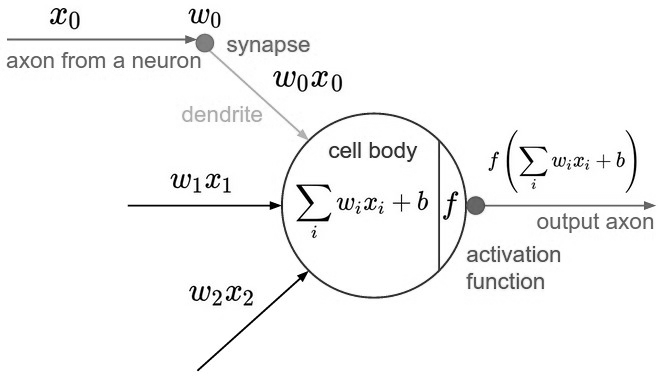
\includegraphics[width=0.75\textwidth]{figures/neuron_model.png}
        \caption[From a biological neuron to a mathematical model: an artificial neural network in its simplest form]{From a biological neuron to a mathematical model in its simplest form: an artificial neural network\protect\footnotemark}
        \label{fig:neuron_model}
    \end{figure}

    \footnotetext{\url{https://cs231n.github.io/neural-networks-1/}}

    In its simplest form, this \gls{nn} is called a \textit{perceptron} or \textit{feed-forward network}, with one input layer and one output node, see Figure~\ref{fig:neuron_model}.
    In this form, the \gls{nn} allows for a generalized variation of a linear function.
    A general perceptron is of the form $(\bar{\boldsymbol{X}},y)$, where $\bar{\boldsymbol{X}}=[x_0,x_1,\ldots,x_d]$ are the \textit{input variables} in vector notation and $y \in \mathbb{R}$  represents the \textit{observed value}.
    The observed value stands for a numerical scalar used for a regression problem, e.g. predicting the price of a house given some numerical input variables such as the number of rooms and square meters.
    In the case of classification, this perceptron allows for binary classification where the observed value is $y$ $\in [-1,+1]$.
    For instance, this can be used to predict whether or not a credit-card transaction was fraudulent given the amount and frequency of the transaction.
    Given the input values $\bar{\boldsymbol{X}}$ and the weights $\bar{\boldsymbol{W}}=[w_0,w_1,\ldots,w_d]$, a result of a linear function is calculated by the following prediction:

    \begin{equation}
        \bar{\boldsymbol{X}}\cdot\bar{\boldsymbol{W}}=\sum_{j=0}^{d}x_j*w_j\label{eq:feed_forward_equation}
    \end{equation}

    Finally, a prediction $\hat{y}$ for $y$, based on the equation~\eqref{eq:feed_forward_equation}, is performed by activating the result making usage of an \textit{activation function}.
    In the case of classification, the \textit{sign activation function} is used to map the prediction $\hat{y}$ to the previously specified range of $[-1,1]$.
    After the activation of the output value, an error between the prediction and the actual outcome can be calculated, $E(\bar{\boldsymbol{X}}) = y - \hat{y}$~\citep[\p{5ff}]{aggarwal_neural_2018}.
    If the error $E(\bar{\boldsymbol{X}})$ is non-zero, the weights must be adapted in order to perform a closer prediction for the next time.
    By optimizing the error function or \textit{loss function}, the classification error is reduced.
    The optimization process is also known as \textit{gradient descent} which updates the weights according to the negative direction of the function's gradient with respect to each input~\citep[\p{7}]{aggarwal_neural_2018} and is formally described by the following notation:

    \begin{equation}
        \bar{\boldsymbol{W}} \Leftarrow \bar{\boldsymbol{W}} + \alpha E(\bar{\boldsymbol{X}})\bar{\boldsymbol{X}}\label{eq:weight_adjusting}
    \end{equation}

    The parameter $\alpha$ is the \textit{learning rate} which defines how large the updates to the weights should be.
    A large value of $\alpha$ allows for faster convergence to a local optimum with the accompanying risk of never reaching one at all.
    On the other hand, a small value steadily approaches the optima but takes longer.


    As the perceptron represents a linear function, it must not only learn the slope but also the intercept, the invariant part.
    The intercept value is also called \textit{bias} and is especially necessary in scenarios where all the features are centred around the mean and the values of the target class are not centred around the origin~\citep[\p{6}]{aggarwal_neural_2018}.
    To solve this issue, the bias variable is introduced to the perceptron as an additional neuron and an extra weight which is adjusted during the error optimization process.
    This additional neuron solely has the purpose to feed the scalar 1 to the output node and by refining the weight in between, the intercept value is learned.
    By incorporating the bias neuron, the following equation emerges:

    \begin{equation}
        \bar{\boldsymbol{X}}\cdot\bar{\boldsymbol{W}} + b=\sum_{j=0}^{d}x_j*w_j + b\label{eq:linear_function_equation}
    \end{equation}

    \subsection{Activation Functions}
    In general, activation functions play an important role in \glspl{nn} as they define the output values of neurons.
    However, they are especially significant for \glspl{mlp} as they determine the modelling power of the network.
    By using nonlinear functions, more sophisticated compositions can be created as they are not reducible to simple perceptrons~\citep[\p{13}]{aggarwal_neural_2018}.

    Apart from the previously noted sign function, other activation functions exist as well and a selection of them can be observed in Figure~\ref{fig:activation_functions}.
    As mentioned in subsection~\ref{subsec:the-basic-architecture-of-neural-networks}, the sign function allows for binary classification of class labels.
    Furthermore, to enable the evaluation of the certitude of a \gls{nn}, the \textit{sigmoid activation function} is employed instead.
    Using this function allows for a mapping of the pre-activated value to a range between $[0,1]$, enabling an estimation of the network's certainty.
    Therefore, $\hat{y}$ indicates the likeliness of an input being a certain target class.
    In contrast to this, the \textit{identity activation function} is used to predict real numbers.
    By using the identity function, the \gls{nn} is equivalent to the \textit{least-squares regression} algorithm.
    An important property that all activation functions have in common is monotonicity and besides the identity function, they also "\textit{saturate at large absolute values at which increasing further does not change the activation much.}"\citep[\p{13}]{aggarwal_neural_2018}

    \begin{figure}[h]
        \centering
        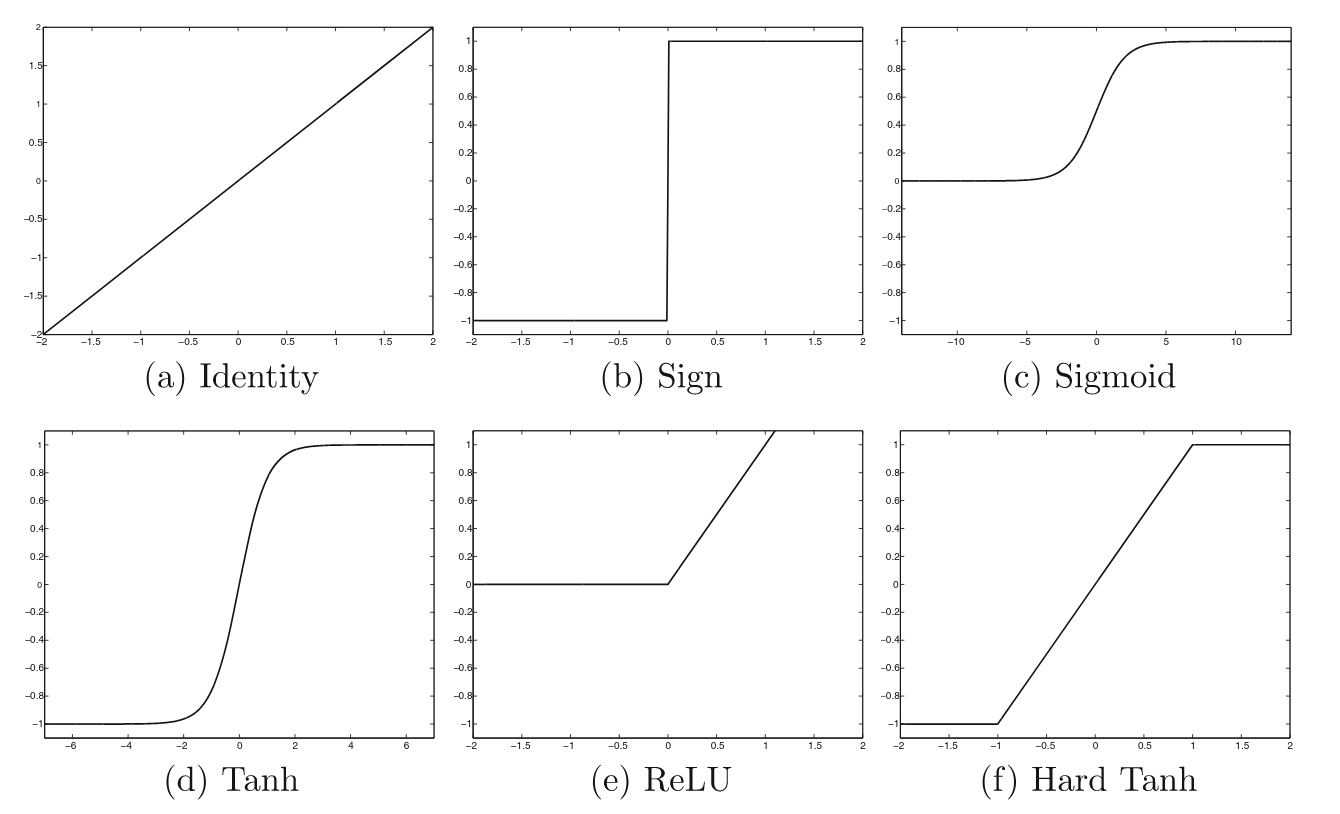
\includegraphics[width=\textwidth]{figures/various_activation_functions.png}
        \caption[Various activation functions and their relationship between the domain and the codomain]{Various activation functions and their relationship between the domain and the codomain\protect\footnotemark}
        \label{fig:activation_functions}
    \end{figure}

    \footnotetext{\cite[\p{13}]{aggarwal_neural_2018}}

    Activation functions are applied on the pre-activated value and therefore a formal notation of $\hat{y}$ is denoted by $\hat{y}=\phi(\bar{\boldsymbol{W}}\cdot\bar{\boldsymbol{X}})$.
    Over the course of the advancement of \gls{nn}, initial activation functions such as the Sigmoid and the \textit{Tangens-Hyperbolicus} activation function have been replaced by piecewise linear functions such as the \textit{\gls{relu} activation function}.

    \begin{align*}
        &\text{Sigmoid: } &  \phi(v) & = \frac{1}{1+e^{-v}} \\
        &\text{Tangens-Hyperbolicus: } &  \phi(v) &= \frac{e^{2v}-1}{e^{2v}+1} \\
        &\text{\gls{relu}: } &  \phi(v)& = \vphantom{\frac11} \max\{v,0\}
    \end{align*}

    This is due to the fact that it facilitates the training process of \glspl{mlp} as they are less expensive to compute.

    \subsection{Loss Functions}\label{subsec:loss-functions}
    In subsection~\ref{subsec:the-basic-architecture-of-neural-networks}, a generic loss function $E(\bar{\boldsymbol{X}})$ has been introduced.
    However, depending on the target and the prediction $\hat{y}$, another loss function may be better suited as certain loss functions are more sensitive to errors for classification than for predicting real numbers~\citep[\p{15}]{aggarwal_neural_2018}.
    For instance, regression tasks modelled by \glspl{nn} with an identity activation function commonly use the \textit{squared loss} $(y - \hat{y})^2$ as an error measurement.
    In the case of classification tasks with multiple class labels, output values are normally activated employing the \textit{softmax activation function}~\citep[\p{78}]{goodfellow_deep_2016}, with $\boldsymbol{v}$ being the $n$ pre-activated output values.

    \[
        \text{Softmax: } \sigma(\boldsymbol{v})_i = \frac{e^{v_i}}{\sum_{j=0}^{n}e^{v_j}}
    \]

    This function allows for a probabilistic output which means that it maps the pre-activated values to a probability distribution.
    Since the output of the softmax function is a vector of probabilities instead of a scalar value, a different loss function is needed as well.
    Additionally, classification tasks can have binary or categorical/multiple targets which further define and differentiate which loss function will be used.

    For binary targets, different combinations of activation and loss functions can be utilized to obtain the same result for prediction.
    For example, binary targets are classified by means of \textit{logistic regression} which makes usage of the identity activation function to predict $\hat{y}$.
    A loss function for this prediction is defined by the following equation:

    \begin{equation}
        L=\text{log}(1+e^{-y\cdot\hat{y}})
    \end{equation}

    A further option is to simply use the sigmoid activation function which maps the output $\hat{y}$ between $0 \text{ and } 1$.
    Under the assumption that the observed value $y$ is normalized between $-1 \text{ and } 1$, the negative logarithm of $|\frac{y}{2}-\frac{1}{2}+\hat{y}|$ is deployed as a loss function~\citep[\p{15}]{aggarwal_neural_2018}.
    This loss function provides a measurement on how likely it is that the target has correctly been classified.

    Concerning categorical targets, post-activated values $\hat{y}_0,\ldots,\hat{y}_n$ are examined one by one.
    The loss for the $i$th prediction is given by the following equation:

    \begin{equation}
        L=-\text{log}(\hat{y}_i)
    \end{equation}

    This definition is known as the \textit{cross-entropy loss} and represents the extension of logistic regression~\citep[\p{15}]{aggarwal_neural_2018}.


    \section{Multi-Layer Neural Networks}
    Comparing a simple perceptron to an \gls{mlp}, the major difference is the employment of multiple layers, the so-called \textit{hidden layers}.
    Instead of a perceptron where all computations are visible, hidden layers in an \gls{mlp} hide the computations~\citep[\p{17}]{aggarwal_neural_2018}.
    However, the \gls{mlp} still is a feed-forward network and the perceptron, as well as the \gls{mlp}, can both be denoted as a \textit{directed acyclic graph}.
    The additional layers in an \gls{mlp} can be described as a composition of multiple functions, in opposition to a perceptron where the input is directly transmitted to the output layer.
    By composing the additional layers via chain-like structures, the input is fed through multiple layers before it allows a prediction of $\hat{y}$.
    For instance, an \gls{mlp} with three layers approximates the function $f(\bar{\boldsymbol{X}})$ by chaining three functions $f^{(3)}(f^{(2)}(f^{(1)}(\bar{\boldsymbol{X}})))$ together for a prediction~\citep[\p{163f}]{goodfellow_deep_2016}.

    The amount of layers or rather the length of the chain is known as the depth of a \gls{nn}/an \gls{mlp} which also established the name \textit{deep learning} (\gls{dl}).
    As aforementioned in the introduction to chapter~\ref{ch:deep-reinforcement-learning}, only \glspl{mlp} with their ability to chain multiple functions enable the approximation of a complex value function in a high dimensional state-space.

    \begin{figure}[h]
        \vspace{0.5cm}
        \centering
        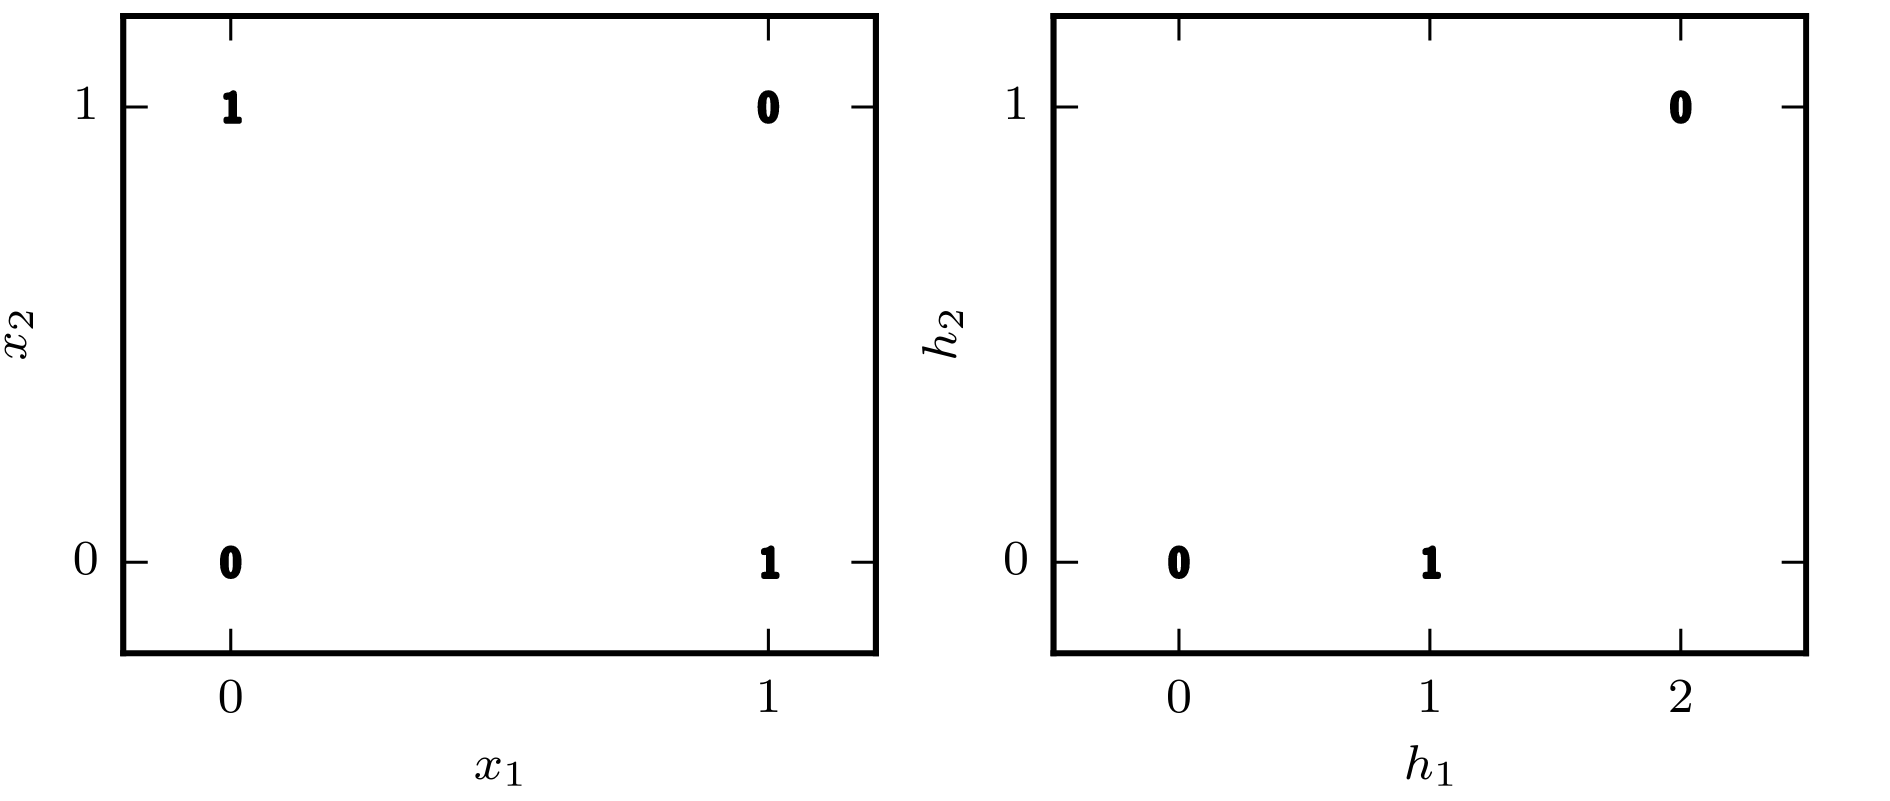
\includegraphics[width=0.75\textwidth]{figures/xor_problem.png}
        \caption[The XOR problem]{The XOR problem with the left plot being the original space using a perceptron and the right plot being the learned space using an \gls{mlp}\protect\footnotemark}
        \label{fig:xor_problem}
    \end{figure}

    \footnotetext{\cite[\p{168}]{goodfellow_deep_2016}}
    The reason why \glspl{mlp} are the preferred choice instead of a perceptron is illustrated by an example of a \gls{nn} which should estimate a model for the logical operator XOR, the "exclusive or".
    In detail, the XOR functions takes two binary values $x_0,x_1$ and returns 1 if $x_1 \neq x_2$ and 0 otherwise.
    This described behaviour is also known as the target function $f^*(\bar{\boldsymbol{X}})$ of the XOR function the \gls{nn} should approximate.
    Observing Figure~\ref{fig:xor_problem}, the learned linear function of a perceptron would no be able to correctly implement the XOR function.
    Applying the model learned by the perceptron to the left, the original space, an approximated linear function cannot separate these values and thus would not be able to return the correct $y$.
    This is also known under the term of \textit{linear separability}.
    However, after transforming the original space with the help of a hidden layer and a nonlinear activation function (e.g. \gls{relu}) to the space on the right side, the XOR function can be solved as the space is now linear separable~\citep[\p{166ff}; \p{32ff}]{goodfellow_deep_2016,aggarwal_neural_2018}.
    This shows that an \gls{mlp} allows for much more complex function approximation.
    With the newly introduced capability, the learning process mentioned in equation~\ref{eq:weight_adjusting} in section~\ref{subsec:the-basic-architecture-of-neural-networks} is not applicable anymore.
    Instead, a new algorithm named \textit{backpropagation} was introduced by \citeauthor{rumelhart_learning_1986} which can be looked up either in \citet[\p{21}]{aggarwal_neural_2018} or in a more formal way in \citet[\p{197}]{goodfellow_deep_2016}.

%\subsection{(Optional)Convolutional Neural Networks}

%\subsection{(Optional)Variational Auto Encoders}


    \section{Deep Learning Approach in Reinforcement Learning}
    The advancements of \gls{dl} over the last couple of years, starting around 2010, allowed the domain of \gls{rl} to evolve as well.
    Especially through the previously mentioned combination of these two fields and the new creation of the \gls{drl} domain, many astonishing accomplishments were achieved~\citep{francois-lavet_introduction_2018}.
    A summary of four different achievements which were selected by \citet[\p{374}]{aggarwal_neural_2018} are listed in the following enumeration.

    \begin{itemize}
        \item Video games are a classical example where \gls{drl} excelled over the course of the last few years.
        Especially, games from the Atari 2600 gaming console are famous environments where \gls{drl} algorithms are applied, receiving only the raw pixels as an input.
        Based on the pixels, a state-representation is formed on which the agent takes actions, makes mistakes, gains experience and finally improves its decision making.
        This procedure is equivalent to the traditional \gls{rl} approach known from chapter~\ref{ch:reinforcement-learning-background}.
        However, it is now applied to a much richer state-space and thanks to \gls{dl}, the agent can surpass humans in these games~\citep{mnih_playing_2013,schulman_trust_2015}.
        Furthermore, the reason why video games are so popular even in modern \gls{rl} is that they function as simulations of real-life microcosms that are perfectly suitable for testing algorithms before being applied in the real world.

        \item   Another very famous breakthrough occurred in 2016 when an algorithm by the name \textit{AlphaGo}~\citep{silver_mastering_2017} defeated the top-ranked players in the board game Go.
        The reason why this event was so remarkable is that Go is a very complex game and being good at it takes a lot of human-like intuition.
        Additionally, the state space is very large when compared to other board games such as e.g. chess.
        However, it was the unconventional learning process which made AlphaGo well known as it improved itself by obtaining experience by playing against another version of itself.

        \item   \gls{drl} is also considered a viable option for self-driving cars.
        Although a more common approach to this problem is the utilization of supervised learning, the usage of various car sensors for decision making allows these automated cars to have a lower error rate when compared to humans.
        \item   Another important domain where \gls{drl} plays a key factor is the creation of self-learning robots.
        Here, the difficulty relies on teaching a robot basic human-like motions such as walking.
        Fortunately, the task of teaching a robot to walk can be described in the \gls{rl} framework as the robot's goal is to reach a given position as fast as possible.
        The robot's state is a description of its available limbs and motors in a continuous space.
        Therefore, \gls{dl} techniques must be applied as well to reach good performance which does not only allow the robot to learn how to walk but also how to roll and crawl.
    \end{itemize}

    All of these accomplishments are based on different \gls{drl} approaches.
    However, an exhaustive explanation of each of these algorithms would go beyond the scope of this thesis.
    Therefore, solely an overview is provided by Figure~\ref{fig:drl_taxonomy} and solely \gls{ppo} is introduced.
    For further information, the paper by \citeauthor{francois-lavet_introduction_2018} is recommended.

    \begin{figure}[h]
        \centering
        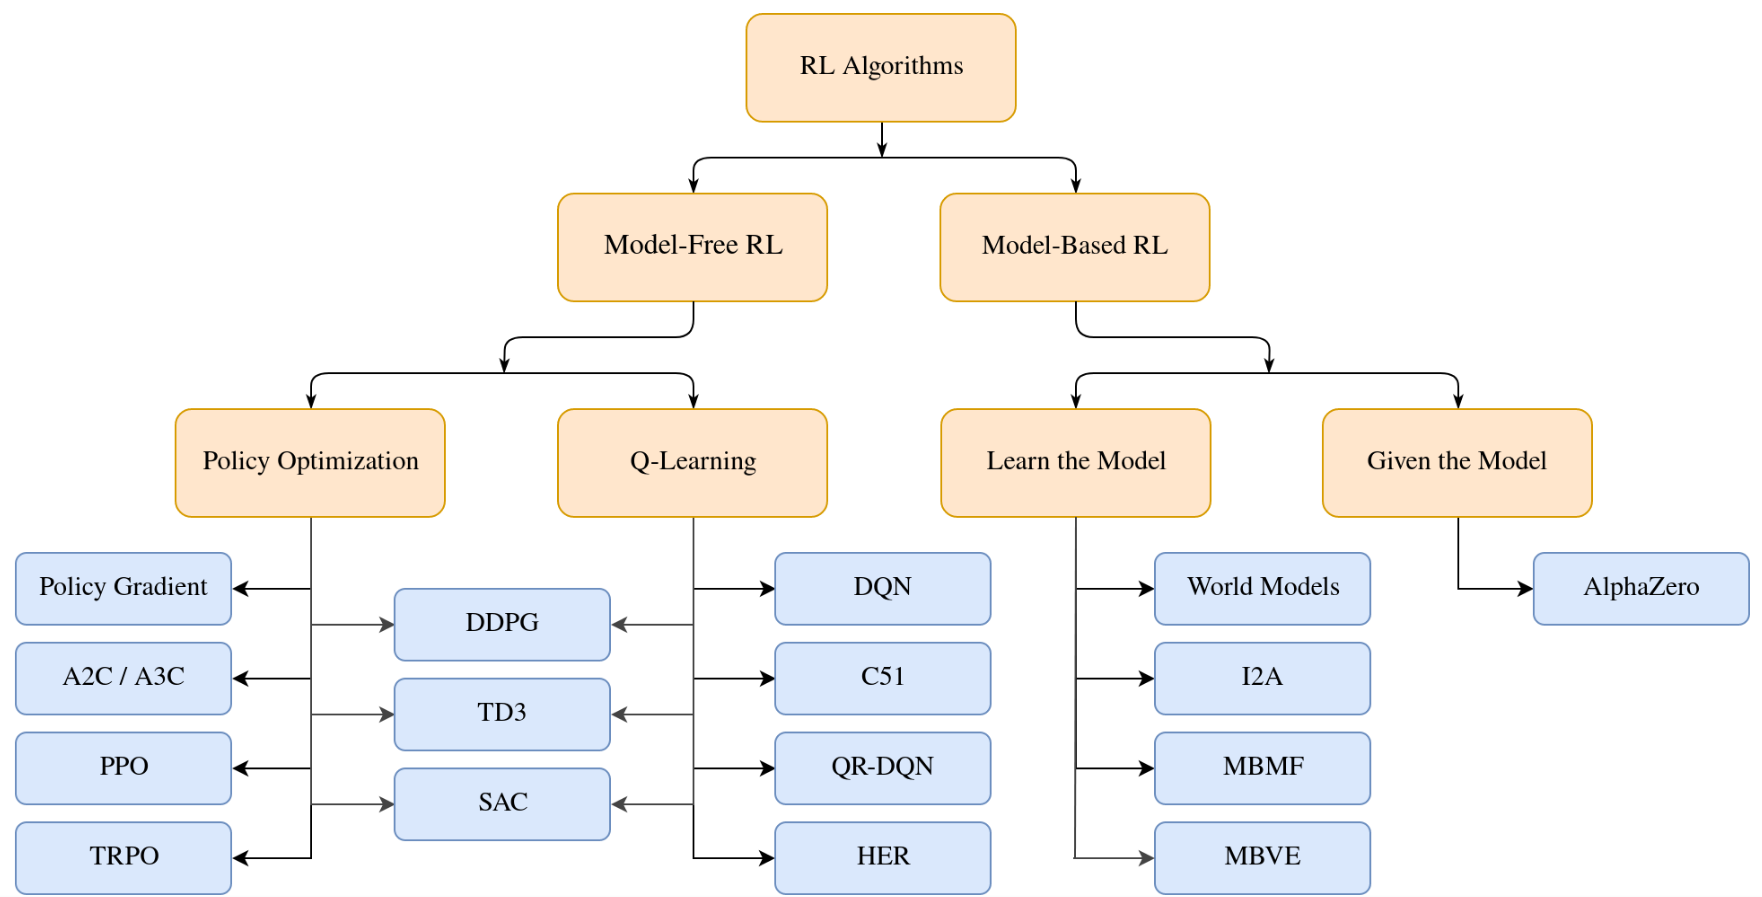
\includegraphics[width=\textwidth]{figures/drl_taxonomy.png}
        \caption[A non-exhaustive taxonomy of \gls{drl} algorithms]{A non-exhaustive taxonomy of \gls{drl} algorithms\protect\footnotemark}
        \label{fig:drl_taxonomy}
    \end{figure}

    \footnotetext{\url{https://spinningup.openai.com/en/latest/spinningup/rl_intro2.html}}


    \section{Proximal Policy Optimization}\label{sec:proximal-policy-optimization}
    \gls{ppo} belongs to the family of policy gradient~\eqref{sec:policy-gradient-methods}, model-free based methods (see Figure~\ref{fig:drl_taxonomy}) that switches between gathering data by interacting with the environment and a stochastic gradient ascent optimization process of a surrogate target function.
    In comparison to equation~\ref{eq:parameter_update}, \citeauthor{schulman_proximal_2017} denote the estimator for the gradient slightly different:

    \begin{equation}
        \hat{g}=\hat{\mathbb{E}}_t \bigg [\nabla_\theta \text{log}\pi_\theta(a_t|s_t)\hat{A}_t\bigg]\label{eq:policy_gradient_method_maximization}
    \end{equation}

    Here, $\hat{A}_t$ estimates an advantage function for a time-step $t$ where the advantage function describes
    how good an action $a$ might be, given the expected return if the policy $\pi$ is followed directly.
    In general, it is denoted by $A^\pi(s,a)=Q^\pi(s,a)-V^\pi(s)$ for a given policy, according to \citeauthor{francois-lavet_introduction_2018}.
    Furthermore, $\hat{\mathbb{E}}_t[\cdot]$ is the empirical mean over some batch samples of interactions with the environment.

    In software, the estimation of the gradient $\hat{g}$ is obtained by creating a similar objective function that acts as the estimator.
    This is done by differentiating the following loss function:

    \begin{equation}
        L^{PG}(\theta)=\hat{\mathbb{E}}_t\bigg [\text{log}\pi(a_t|s_t)\hat{A}_t\bigg]\label{eq:no_clip_no_penalty}
    \end{equation}

    Additionally, \gls{ppo} is based on an idea named \gls{trpo} where objective function~\ref{eq:policy_gradient_method_maximization} is replaced by a surrogate objective~\eqref{eq:trpo_optimization} with an additional constraint~\eqref{eq:trpo_constraint} on the update size of the policy~\citep{schulman_trust_2015}.

    \begin{equation}
        \hat{\mathbb{E}}_t\bigg [\frac{\pi_\theta(a_t|s_t)}{\pi_{\theta_{\text{old}}}(a_t|s_t)}\hat{A}_t\bigg]\label{eq:trpo_optimization}
    \end{equation}
    \begin{equation}
        \hat{\mathbb{E}}_t\bigg [\text{KL}[\pi_{\theta_{\text{old}}}(\cdot|s_t),\pi_{\theta}(\cdot|s_t)]\bigg]\leq\delta\label{eq:trpo_constraint}
    \end{equation}

    Instead of the constraint~\ref{eq:trpo_constraint}, a penalty is sometimes integrated with a corresponding weighting as well, combining the equations~\ref{eq:trpo_optimization} and~\ref{eq:trpo_constraint}.
    Furthermore, KL in equation~\ref{eq:trpo_constraint} stands for the Kullback-Leibler divergence.

    With the ratio $r_t(\theta)=\frac{\pi_\theta(a_t|s_t)}{\pi_{\theta_{\text{old}}}(a_t|s_t)}\hat{A}_t$ the main objective for \gls{ppo} can now be constructed:

    \begin{equation}
        L^{CLIP}(\theta)=\hat{\mathbb{E}}_t\bigg[\text{min}(r_t(\theta)\hat{A}_t,\text{clip}(r_t(\theta),1-\epsilon,1+\epsilon)\hat{A}_t)\bigg]\label{eq:ppo_clip}
    \end{equation}

    The main objective of the \gls{ppo} differs mainly from the surrogate objective of \gls{trpo}~\eqref{eq:trpo_optimization} as it does not allow for excessively large changes to the policy.
    This is done by clipping the initial objective, if the probability ratio $r_t$ moves too far away from 1 and whether or not the advantage $\hat{A}_t$ is negative or positive.
    Thus, a restriction is placed upon the incentive to move outside of $[1-\epsilon,1+\epsilon]$, with $\epsilon$ being a hyperparameter.
    Moreover, the minimum of the equation~\ref{eq:ppo_clip} functions as a lower bound for the objective~\ref{eq:trpo_optimization}.

    Referring to the results of \citeauthor{francois-lavet_introduction_2018} where the authors tried different surrogate objectives on seven environments with three different seeds, clipping the objective~\eqref{eq:ppo_clip} with an $\epsilon=0.2$ resulted in the best normalized, averaged score of 0.82.
    By using different $\epsilon \in [0.1,0.3]$, the score varies between $[0.70,0.82]$ whereas KL-penalized objectives achieved scores between $[0.62,0.72]$ and a non clipped and penalized objective~\eqref{eq:no_clip_no_penalty} performed the worst with an average score of $-0.39$~\citep[see Table 1]{francois-lavet_introduction_2018}.

    When comparing \gls{ppo} algorithms to similar approaches such as \gls{trpo}, \citeauthor{francois-lavet_introduction_2018} list the following advantages:

    \begin{quote}
        "[T]hey are much simpler to implement, more general and have better sample complexity (empirically). [Furthermore,] \ldots PPO outperforms other online policy gradient methods, and overall strikes a favorable balance between sample complexity, simplicity, and wall-time."

        \hfill ~\citep[\p{1}]{francois-lavet_introduction_2018}
    \end{quote}

    In \gls{drl} applications where \gls{nn} share parameters between a value function and a policy, they both must be combined to form one uniform loss function.
    Additionally, to construct the objective which \gls{ppo} tries to maximize, a bonus in the form of an entropy is added to ensure enough exploration, resulting in a final target that is given by the following equation:

    \begin{equation}
        L_t^{CLIP+VF+S}(\theta) = \hat{\mathbb{E}}_t\bigg[L_t^{CLIP}(\theta) - c_1L_t^{VF}(\theta) + c_2S[\pi_\theta](s_t)\bigg]\label{eq:ppo_objective}
    \end{equation}

    In this equation, $S$ is the bonus in form of an entropy, $L_t^{VF}$ denotes the squared-error loss $(V_\theta(s_t)-V_t^{\text{targ}})^2$ and $c_1,c_2$ are coefficients which control the influence of these two terms.
    Implementing and optimizing the objective~\ref{eq:ppo_objective} is carried out by following the policy and collecting samples of interactions with the environment for $T$ time-steps.
    The gathered data is then used to apply an update to~\ref{eq:ppo_objective}.
    Additionally, the advantage function, needed for objective~\ref{eq:ppo_clip}, is approximated by an estimator which only considers $T$ time-steps with an index $t\in [0,T]$ as well and is denoted as follows:

    \begin{equation}
        \hat{A}_t=-V(s_t)+r_t+\gamma r_{t+1} + \dots + \gamma^{T-t+1}r_{T-1} + \gamma^{T-t}V(s_T)\label{eq:advantage_estimator}
    \end{equation}

    The \gls{ppo} algorithm, shown below~\eqref{alg:ppo}, puts theory into practice where in each iteration, $N$ workers gather data for $T$ time-steps, calculate the loss with these $NT$ time-steps and apply the just calculated loss in minibatches for $K$ epochs~\citep{francois-lavet_introduction_2018}.
    \newpage
    \begin{algorithm}
        \caption[\gls{ppo}, Actor-Critic Style]{\gls{ppo}, Actor-Critic Style\protect\footnotemark}
        \label{alg:ppo}
        \SetKw{Run}{run}
        \SetKw{Comp}{compute}
        \SetKw{Opt}{optimize}
        \SetKw{Update}{update}

        \For{
        $iteration=1,2,\dots$}{
        \For{$actor=1,2,\dots,N$}{
        \Run{policy $\pi_{\theta_\text{old}}$ in environment for $T$ time-steps}\;
        \Comp{advantage estimates $\hat{A}_1,\hat{A}_2,\dots,\hat{A}_T$}\;
        }
            \Opt{surrogate $L$ wrt $\theta$, with $K$ epochs and minibatch size $M \leq NT$}\;
            \Update{$\theta_\text{old}\leftarrow \theta$}\;
        }



    \end{algorithm}

    \footnotetext{\citep[\p{5}]{schulman_proximal_2017}}

    \glsresetall


    \chapter{Intrinsic Motivation in Reinforcement Learning}\label{ch:intrinsic-motivation-in-reinforcement-learning}
    The idea of including \gls{im} into the \gls{rl} framework has been around since early 1990 as in realistic environments extrinsic rewards occur rather rare and thus quick progress by an agent cannot be expected.
    With its roots deeply involved in psychology, \gls{im} was initially used due to its ability of discovering surprising or novel patterns, enabling an agent to be creative in the sense that it learns non-trivial, new behaviour~\citep{schmidhuber_formal_2010}.
    This phenomenon is based on a discovery from nature as animals were observed to engage in curiosity-driven, exploratory, and playful behaviour despite the fact that they would not obtain a reward or a reinforcement~\citep{white_motivation_1959}.

    This chapter is started by introducing the psychological aspects of \gls{im} as well as the term motivation in general and is continued with the role of \gls{im} in the \gls{rl} framework.
    Afterwards, current challenges of \gls{rl} which are tackled by \gls{im} are pointed out (see Listing~\ref{enm:challenges} for a summary), and the embedding of \gls{im} in \gls{rl} is presented.
    Finally, this chapter is concluded with the classification of \gls{im} in \gls{rl}: \textit{knowledge acquisition} and \textit{skill learning} where a subdomain of knowledge acquisition is more deeply explored in chapter~\ref{sec:state_of_the_art} as it represents the domain on which the implementation~\eqref{ch:implementation} is based on.


    \section{Natural Human Motivation}

    In a digression to psychology, \gls{im} is described as the natural propensity of humans to gather knowledge and assimilate.
    Activities which are intrinsically motivated are usually carried out because they are enjoyable and interesting.
    Therefore, the reward in \gls{im} relies on the activity itself.
    In opposite to that, \gls{em} reflects external control sources or true self-regulation which may achieve separable outcomes, e.g.\ food or money.
    Motivation, in general, is very unique for different people~\citep{ryan_intrinsic_2000}.
    Not only can it vary in the amount or rather the \textit{level of motivation} a person can have, but the \textit{orientation of motivation} can be different as well.
    The question on the orientation of a person's motivation is very significant since e.g.\ pupils may be very motivated to excel in a subject out of curiosity (\gls{im}) or rather out of the possibility of achieving good grades (\gls{em}) which might yield further positive benefits for them or avoid sanctions.

    Moreover, research pointed out that the quality of performance and experience is dependant on the kind of motivation propelling behaviour.
    For instance, it is shown that \gls{im} allows for an improved learning experience and more creativity.
    On the other side, extrinsic motivated actions might be executed with disinterest, resistance or optionally with an inner acceptance as the action poses an identifiable value~\citep{ryan_intrinsic_2000}.
    Continuing with the previously made example on the pupils' motivation, for instance, it is the teacher's job to promote inherently uninteresting actions by means of extrinsic motivation with a focus on volitional and active forms instead of controlling and passive ones.
    By doing this, the pupils are more likely to identify the action's value such that they internalize the behaviour, allowing for an improved learning experience.

    Finally, \citeauthor{ryan_intrinsic_2000} add a third type of motivation to the taxonomy of natural human motivation, the so-called \textit{amotivation} which describes activities that are perceived as irrelevant.
    Amotivation has different origins such as a feeling of incompetence to carry out a task, an action not yielding any value, or any desired outcome.
    Therefore, the taxonomy of human motivation consists of three branches: amotivation, extrinsic motivation, and intrinsic motivation, ranging "\textit{from amotivation or unwillingness, to passive compliance, to active personal commitment. With increasing internalization (and its associated sense of personal commitment) come[s] greater persistence, more positive self-perceptions, and better quality of engagement.}"~\citep[\p{60f}]{ryan_intrinsic_2000}


    \section{The Role of Intrinsic Motivation in Reinforcement Learning}

    With the help of \gls{im}, existing challenges of \gls{rl} such as abstracting actions or the exploration of the environment should be addressed which were not able to be solved by the promising capabilities of \gls{nn}.
    As mentioned in the~\nameref{sec:problem-description}, in traditional \gls{rl} approaches, the agent is unable to explore the environment in settings where rewards are sparse.
    Furthermore, even in dense environments, the agent's learned behaviour is rather not reusable in similar as well as in completely different tasks.
    This is due to the fact that an agent finds it very challenging to generalize obtained skills and thus is incapable of high-level decision making.
    For instance, \citeauthor{todorov_mujoco_2012} indicate that such a high-level abstraction could be the trajectory of a robot to open a door which consists of low-level actions or rather movements in four directions.

    As earlier described, the idea for \gls{im} in \gls{rl} is derived from nature, especially by the animals' urge for exploration.
    However, a probably better fitting example would be a baby's task to solve existential problems as it best reflects a \gls{rl}-agent in an unknown environment.
    For instance, in order for the baby to avoid hunger or thirst, it has to learn the consequences of its interactions.
    Although immediate needs might be satisfied for some time, the baby continues to explore by conducting different experiments.
    Questions on certain movements of, e.g.\ eyes, fingers, or the tongue and their expected sensory feedback are continually answered.
    Ultimately, this facilitates the baby's ability of prediction which allows for easier planning of actions.
    Furthermore, the baby constantly strives to discover new effects, as it eventually gets bored by the things it already grasps, allowing it to learn very complex behaviour by building on previously gathered knowledge.
    By following this simple algorithm of maximizing the internal joy of discovering or creating new patterns, eventually, the baby might become a computer scientist~\citep{schmidhuber_formal_2010}.
    Concerning \gls{rl}, this process allows an agent to autonomously gather new skills and knowledge which then facilitates the mastering of a novel task.

    Besides the improved exploration, \gls{im} yields other benefits as well.
    For instance, an agent can learn skills incrementally and independently while not being dependant on its given main task.
    Furthermore, the agent can decide on which skill might be adequate for a certain task and thus improve them selectively and additionally it might as well come up with a meaningful state representation.
    This is all possible due to the broader intrinsic reward function and the fact that this spares the necessity of an expert or supervisor.
    Therefore, making learning more flexible and \gls{rl} to generalize more across different environments~\citep{aubret_survey_2019}.

    Additionally to the classification of subfields in \gls{ml} in section~\ref{sec:reinforcement-learning-problem}, \citeauthor{aubret_survey_2019} add a fourth field to the spectrum of learning types, differentiating between reinforced and intrinsically motivated learning (see Table~\ref{tab:type_learning}).
    Therefore, a distinction is drawn depending on whether or not expert supervision is involved which gives feedback.

    \begin{table}
        \centering
        \begin{tabular}{|l|l|l|}
            \hline
            & With \textit{feedback} & Without \textit{feedback} \\
            \hline
            Active  & Reinforcement          & Intrinsic motivation      \\
            \hline
            Passive & Supervised             & Unsupervised              \\
            \hline
        \end{tabular}
        \caption[A taxonomy on the different types of learning]{A taxonomy on the different types of learning\protect\footnotemark}
        \label{tab:type_learning}
    \end{table}

    \footnotetext{\citep[\p{4}]{aubret_survey_2019}}


    \section{Challenges}

    \subsection{Sparse Rewards}\label{subsec:sparse-rewards}

    As noticed in section~\ref{sec:problem-description}, traditional \gls{rl} algorithms perform best in environments which reward the agent densely.
    By using naive exploration approaches, e.g. $\epsilon\text{-greedy}$, good results can be accomplished with an additional option, for instance, to add \textit{Gaussian noise} to the action selection process which further improves exploration~\citep{lillicrap_continuous_2019}.
    However, even these improved exploration methods are incapable to achieve a good performance in sparsely rewarding settings such as \textit{Montezuma's Revenge} which is a typical benchmark for such environments.
    In order for the agent to receive a reward in this game, it has to collect different items such as keys and use them to open doors.
    These events occur rather rarely and thus the agent does not receive immediate feedback concerning the impact of its performed actions, e.g.\ moving in a certain direction.
    Therefore, it is not uncommon that an agent never reaches such a reward, preventing the creation of a good policy~\citep{aubret_survey_2019}.

    This issue can be tackled by shaping a task-specific, intermediary function which rewards densely.
    Hence, additional rewards are created which should point the agent in the right direction.
    Although this approach might work out well, it is usually impractical as in order to craft this function, very high expert knowledge is needed to carefully design this rewarding system.
    Additionally, such functions commonly yield many side effects resulting in unexpected errors as the agent might pick up an undesired behaviour by exploiting the rewarding system.

    \subsection{Building a Good State Representation}\label{subsec:building-a-good-state-representation}

    According to \citeauthor{bohmer_autonomous_2015}, a good state representation allows for good generalization, is low-dimensional, should represent values of a policy truthfully, and be markovian.
    By employing a good representation, the agent's learning process can be considerably accelerated.
    For instance, considering a navigation task, it makes a significant difference whether an agent has to find out its location and the location of its target by accessing non-linear transformed raw pixels or by obtaining the positions directly creating solely the need to check the distance between itself and the target.

    Normally, a state representation can be build using expert knowledge of a specific domain.
    However, not task-specific, hence generic, priors can be used as well with the benefit that these priors can be learned by representation-learning algorithms, creating disentangled, minimal feature spaces~\cite{bengio_representation_2014}.
    In traditional \gls{rl}, the problem of learning a good state representation is exacerbated as in order for the agent to improve, it depends on optimizing the reward signal via backpropagation, thus depending on receiving rewards densely.
    With the additional possible obstacle of noise in the raw state representation, the agent will learn nothing from the interactions it made in a sparse rewarding environment, although they might be rich in information.
    Even if the agent manages to learn a state representation based on a reward signal, the representation will not generalize across different tasks.
    Hence, \gls{im} is a key component as state representations learned through \gls{im} are independent of the actual task and therefore generalizable~\citep{aubret_survey_2019}.

    \subsection{Temporal Abstraction of Actions}\label{subsec:temporal-abstraction-of-actions}

    In the temporal abstraction of actions, a sequence of low-level actions is summarized with a so-called \textit{intra-option policy} that is referenced to a high-level action.
    Therefore, a high-level action or a so-called \textit{option} consists of multiple low-level actions or rather other options.
    By choosing an option in a certain state, the intra-option policy defines which low-level actions must be carried out in each subsequent state until the high-level action is completely carried out.
    Furthermore, the sequence length of these actions is usually fixed~\citep{aubret_survey_2019}.
    By utilizing these abstractions, the learning process can be sped up significantly.
    An additional consequence of allowing these abstractions is that the problem of delayed rewards, described in section~\ref{sec:reinforcement-learning-problem}, is tackled as the option can be directly credited.
    \citeauthor{aubret_survey_2019} describe this with the following example:

    \begin{quote}
        "[L]et us assume that a robot is trying to reach a cake on a table which is far from the robot.
        If the robot has an option \texttt{get to the table} and follows it, the robot will then only have to take the cake to be rewarded.
        Then it will be easy to associate the acquisition of the cake (the reward) to the option \texttt{get to the table}.
        In contrast, if the robot has to learn to handle each of its joints (low-level or primitives actions), it will be difficult to determine which action is responsible for the acquisition of the cake, among all executed actions."

        \hfill~\cite[\p{5f}]{aubret_survey_2019}
    \end{quote}

    Another benefit of temporal abstractions of actions is that they allow for better exploration.
    Similarly to the previously made example, an exploration task can easily be combined to an option enabling it to immediately receive a reward and therefore "making a sparse reward function dense".
    In order to obtain such an intra-option policy, there are two options: define it manually using expert knowledge or learn it using a reward function.
    However, the latter has the problem that the learned options are not generalizable across multiple tasks and hence are useless for exploration tasks~\citep{aubret_survey_2019}.
    Similar to the problem of~\nameref{subsec:building-a-good-state-representation}, by using \gls{im} this challenge can be tackled.

    \subsection{Building a Curriculum}\label{subsec:building-a-curriculum}
    The challenge of building a curriculum is concerned with structuring tasks in a multi-task \gls{rl} scenario, a scenario where an agent has to solve multiple tasks at once.
    In such scenarios, a so-called \textit{curriculum} is employed that acts as a schedule defining the order in which different tasks should be solved.
    This idea stems from the observation that incrementally building upon gathered knowledge from similar but less complex tasks facilitates mastering more difficult ones~\citep{aubret_survey_2019}.

    For instance, a general task for an agent could be that it has to store objects such as cubes in boxes.
    However, this task can be divided in subtasks such as grabbing the cube and then putting it into a box.
    By splitting up this task into the two subtasks, the agent can take advantage of the prior learnt skill of grabbing a cube for the task of storing it in a box.
    Without this differentiation, the agent might be unable to ever fulfil the general task as it would take the agent a long list of subsequent actions or rather joint movements to succeed.

    Usually, standard methods for decomposing a general task mostly rely on expert knowledge which unfortunately always goes along with the inability to scale and generalize well and thus \gls{im} finds its application to solve this issue as it does not only speed up the learning process but also facilitate exploration.


    \section{Classification}

    Concerning the classification of \gls{im} in \gls{rl}, the authors \citeauthor{aubret_survey_2019} propose a new categorization, differentiating between \textit{knowledge acquisition} and \textit{skill learning}.
    With this separation, emphasis is laid on skill abstraction and skill acquisition.

    Concerning the motivation based on \textbf{knowledge acquisition}, the agent's internal goal is to gather new knowledge about its surroundings.
    In this scenario, knowledge is described as its ability to e.g.\ control the environment, understand occurring processes, explore unknown areas, or assess proximity.
    Based on this definition, building an agent with this motivation can greatly improve exploration in settings with sparse rewards.
    This is usually done by giving an agent a feeling for state novelty or information gain which poses an intrinsic reward which it tries to maximize.
    Another benefit yields the idea of empowerment which means that an agent is rewarded by \gls{im} whenever it approaches an area that it can control.
    Finally, this motivation might allow the agent to create a relevant state representation and thus this branch is concerned with the challenges described in subsection~\ref{subsec:sparse-rewards} and~\ref{subsec:building-a-good-state-representation}.

    The second branch, concerning motivation based on \textbf{skill learning}, is described as the ability of an agent to efficiently acquire skills that are task-independent and preferably reusable.
    Here, one idea evolves around the ability of abstracting skills in order for an agent to learn them or rather creating a representation of different skills which challenges the introduced problem of subsection~\ref{subsec:temporal-abstraction-of-actions}.
    Finally, choosing the best-suited skills to fulfil a given task and the order in which they should be obtained is another \gls{im} that can tackle the challenge mentioned in subsection~\ref{subsec:building-a-curriculum}.

    An overview of the just described classification with practical approaches given can be observed in Table~\ref{tab:clasification_im_rl}.

\newpage
    \begin{table}[h]
        \centering
        \begin{tabular}{l}
            \hline
            \multicolumn{1}{|c|}{\textbf{Knowledge Acquisition}}                                                                                                            \\ \hline
            \multicolumn{1}{|l|}{\textbf{Exploration}}                                                                                                                      \\ \hline
            \multicolumn{1}{|l|}{\begin{tabular}[c]{@{}l@{}}~\nameref{sec:prediction-error}\\~\nameref{sec:state-novelty}\\~Novelty as Discrepancy towards other States\footnotemark[3]\\~\nameref{sec:information-gain}\end{tabular}} \\ \hline
            \multicolumn{1}{|l|}{\textbf{Empowerment}}                                                                                                                      \\ \hline
            \multicolumn{1}{|l|}{\textbf{Learning a Relevant State Representation}}                                                                                         \\ \hline
            \multicolumn{1}{|l|}{\begin{tabular}[c]{@{}l@{}}State Space as as Measure of Distance\\ One Feature for one Object of Interaction\end{tabular}}                 \\ \hline
                                                                                                                                                                            \\ \hline
            \multicolumn{1}{|c|}{\textbf{Skill Learning}}                                                                                                                   \\ \hline
            \multicolumn{1}{|l|}{\textbf{Skill Abstraction}}                                                                                                                \\ \hline
            \multicolumn{1}{|l|}{\begin{tabular}[c]{@{}l@{}}Building the Goal Space from the State Space\\ Mutual Information between Goals and Trajectories\end{tabular}}  \\ \hline
            \multicolumn{1}{|l|}{\textbf{Curriculum Learning}}                                                                                                              \\ \hline
            \multicolumn{1}{|l|}{\begin{tabular}[c]{@{}l@{}}Goal Sampling\\ Multi-Armed Bandit\\ Adversarial Training\end{tabular}}                                         \\ \hline
        \end{tabular}
        \caption[Classification of \glspl{im} in \gls{rl}]{Classification of \glspl{im} in \gls{rl}\protect\footnotemark[2]}
        \label{tab:clasification_im_rl}
    \end{table}
    \footnotetext[2]{\citep[\p{9}]{aubret_survey_2019}}
    \footnotetext[3]{Continuing, \citeauthor{aubret_survey_2019} unite state novelty and novelty as discrepancy towards other states}

    \section{Embedding Intrinsic Motivation into the Reinforcement Learning Framework}\label{sec:embeddingglsinto-theglsframework}

    In order to embed \gls{im} into \gls{rl} a new framework from \citeauthor{singh_intrinsically_2010} is considered, splitting the reward signal into primary and secondary rewards.
    The primary reward signal represents the standard one whereas the secondary reward describes a local reward signal which value is similarly computed as the value function~\eqref{eq:quality_function} denoted in section~\ref{sec:functions-to-improve-the-policy}.
    Additionally, the representation of the \gls{rl} framework as a \gls{mdp} is reconsidered as well.
    Instead of describing the agent's surroundings traditionally, they suggested a division of the environment into two separate parts: the \textit{external part} and the \textit{internal part}, where the external part reflects the environment of the agent where it has to complete its assigned task and the internal part calculates the intrinsic reward based on previously made interactions~\citep{aubret_survey_2019}.

    The newly adapted \gls{rl} framework can be observed in Figure~\ref{fig:adapted_rl_framework}.
    Here, the critic describes the part which computes the reward in either way and assigns the credit to the made actions.
    Additionally, the state now includes sensations optionally combined with the agent's performed actions.
    However, the left panel yet describes the traditional \gls{rl} framework in a slightly different notation to the one presented in section~\ref{sec:markov-decision-processes} whereas the right panel includes the new refinements where all rewards come from the internal part~\citep{singh_intrinsically_2010}.

    \begin{figure}[h]
        \centering
        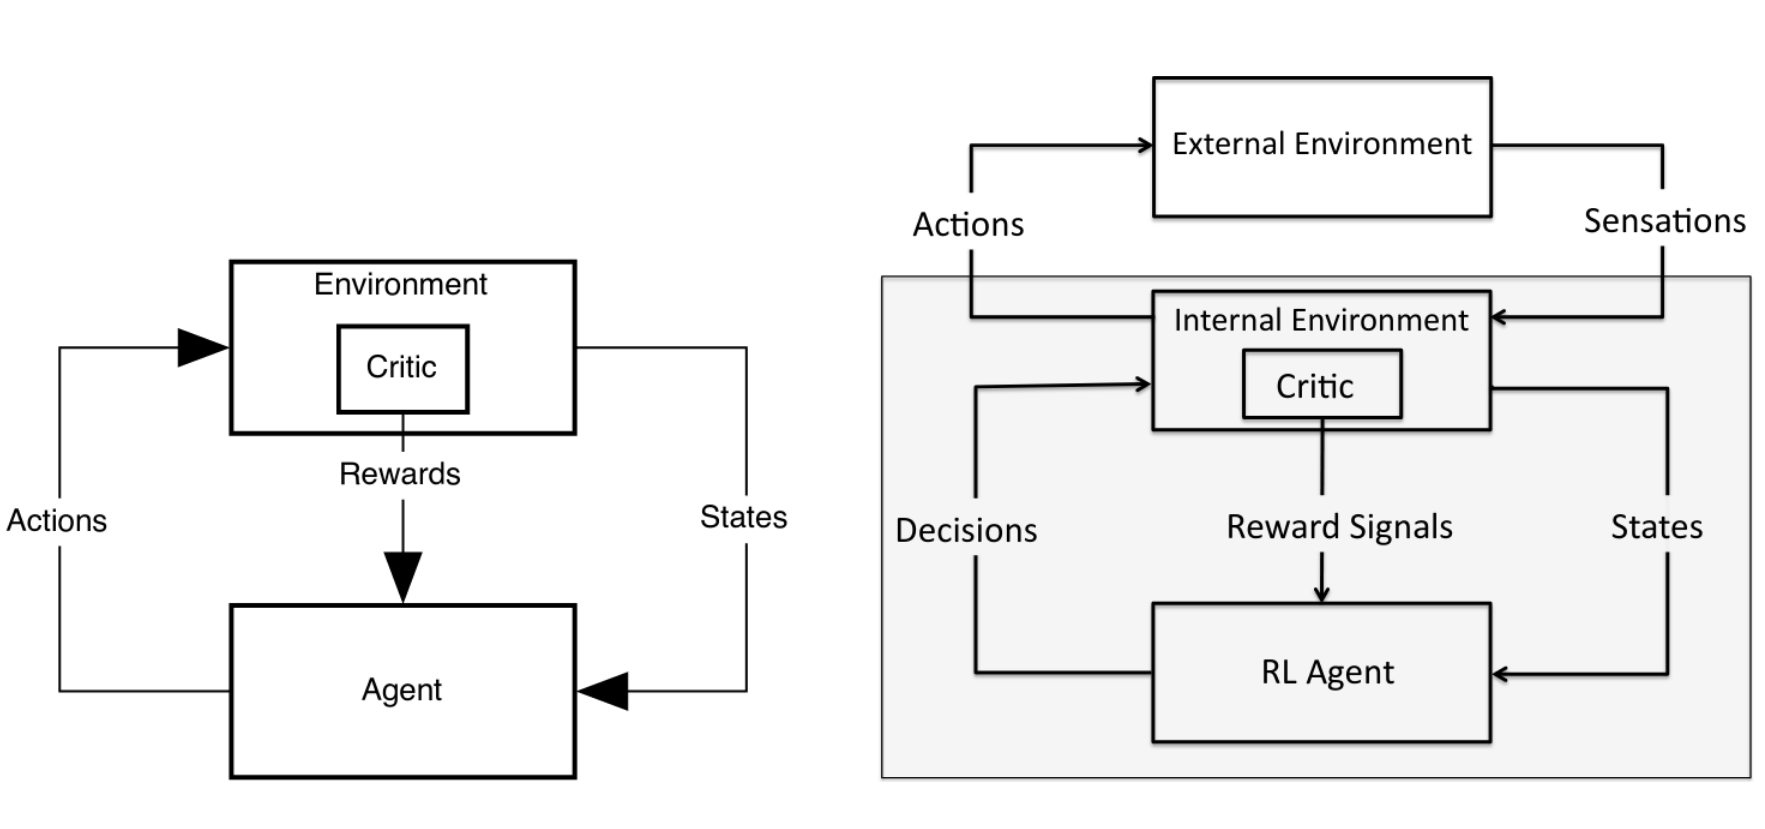
\includegraphics[width=\textwidth]{figures/adapted_rl_framework.png}
        \caption[Adapting the classic \gls{rl} framework to incorporate \gls{im}]{Adapting the classic \gls{rl} framework to incorporate \gls{im}\protect\footnotemark[4]}
        \label{fig:adapted_rl_framework}
    \end{figure}

    \footnotetext[4]{\citep[\p{2}]{singh_intrinsically_2010}}

    One of the most prominent \gls{im} is curiosity which is deployed because it acts as a meta-skill that allows the agent to easily acquire other behaviour.
    In general, the acquisition of task-unspecific skills by means of \gls{im} allows for more intelligent behaviour making the adapted framework more efficient in serving assigned goals when compared to the traditional one.

    When implementing a \gls{rl} algorithm, there are multiple ways to include an intrinsic reward signal.
    The most common approach is to simply combine the existing extrinsic reward signal $(r_{ext})$ with the new intrinsic one $(r_{int})$ by defining coefficients $\alpha$ and $\beta$.
    Those coefficients serve the purpose of weighting the two signals depending on how important either one should be to the agent.
    As this approach poses the core research question of this thesis, that is, how to optimally combine these two rewards, the equation $r = \alpha r_{int} + \beta r_{ext}$ has already been introduced in section~\ref{sec:expected-results}.
    Additionally, when the intrinsic reward is dependant on the value of the extrinsic one, the sum is solely computed on the level of the value function, i.e. $V(s)=\alpha V_{int}(s) + \beta V_{ext}(s)$ as it is the case in the work of \citeauthor{kim_curiosity-bottleneck_2019-1}
    This work as well as many other exploration based methods such as the paper by \citeauthor{burda_exploration_2018} are discussed in the following chapter.
    Besides that, the papers by \citeauthor{gregor_variational_2016}, \citeauthor{vezhnevets_feudal_2017}, and \citeauthor{huang_learning_2019} are also worth mentioning as they combine extrinsic and intrinsic rewards as well but consider \gls{im} in the context of skill learning which is not a focus of this thesis.


    \chapter{Exploration}\label{sec:state_of_the_art}
    In this chapter only the significant branch of knowledge acquisition through exploration is considered as this thesis builds upon a "\usebibentry{burda_large-scale_2018-1}{title}", a paper published by \citeauthor{burda_large-scale_2018-1}
    Here, emphasis is placed on prediction-error based methods but for completeness other exploration methods based on state novelty or information gain are taken into account as well.
    However, the following list of publications poses only a selection which was chosen mainly based on the performance of these methods or was written by authors who contributed to the underlying paper of this thesis.

    \begin{itemize}
        \item \usebibentry{stadie_incentivizing_2015}{title} (\citeauthor{stadie_incentivizing_2015})
        \item \usebibentry{pathak_curiosity-driven_2017-1}{title} (\citeauthor{pathak_curiosity-driven_2017-1})
        \item \usebibentry{kim_emi_2019}{title} (\citeauthor{kim_emi_2019})
        \item \usebibentry{bellemare_unifying_2016}{title} (\citeauthor{bellemare_unifying_2016})
        \item \usebibentry{burda_exploration_2018}{title} (\citeauthor{burda_exploration_2018})
        \item \usebibentry{kim_curiosity-bottleneck_2019-1}{title} (\citeauthor{kim_emi_2019})
        \item \usebibentry{pathak_self-supervised_2019}{title} (\citeauthor{pathak_self-supervised_2019})
    \end{itemize}

    For a more detailed list, \textit{Table 3} by~\citeauthor{aubret_survey_2019} is recommended.

    By not only considering the approach by \citeauthor{burda_large-scale_2018-1}, this chapter also represents a state-of-the-art review for exploration via \gls{im}.
    Finally, at the end of this chapter "\usebibentry{ecoffet_go-explore_2019}{title}" by \citeauthor{ecoffet_go-explore_2019} is presented which is currently the best performing method to solve the exploration challenge offered by \textit{Montezuma's Revenge} as of August 2020.


    \section{Prediction Error}\label{sec:prediction-error}

    The idea of prediction-error based exploration is to point the agent in a direction where a prediction of the next state based on a state-action tuple is rather difficult.
    Formally, this prediction-error based intrinsic reward\footnote{For uniformity reasons, the Greek letter $\phi$ will be used instead of $g$ throughout this chapter} can be denoted as
    \begin{equation}
        R_{int}=||\phi(s_{t+1})-F(\phi(s_t),a_t)||_2
    \end{equation}
    where $||x||_2$ is the L2 distance or rather the Euclidean distance~\citep{aubret_survey_2019}.
    In this equation, $\phi$ stands for a generic function which encodes the raw state space into space of features and $F$ denotes a \gls{nn} which predicts the following feature space depending on the current encoded state and the taken action.

    In the core paper to this thesis, \citeauthor{burda_large-scale_2018-1} deployed four different encodings for $\phi$ and compared the auxiliary feature spaces in terms of compactness, sufficiency, as well as stability in order to find out whether or not an agent can fulfil tasks when purely driven by \gls{im}.
    Concerning the properties of an encoding function $\phi$, they describe compactness to be low in dimensionality, sufficiency to contain all the relevant information about the environment, and stability to be a stationary function.
    Instead of the previously denoted intrinsic reward, \citeauthor{burda_large-scale_2018-1} used the so-called surprisal:
    \begin{equation}
        R_{int}=-\log p(\phi(s_{t+1})|s_t,a_t)
    \end{equation}
    Regarding the actual encoding functions used for their investigations, they started with the identity function, $\phi(s)=s$, which proved to be very inefficient as it lacked compactness even though the encoding was sufficient and stable.
    Additionally, the prediction-error based on this encoding is probably dominated by irrelevant small details.

    In contrast to that, they introduced so-called \gls{rf} where features are extracted using a random initialized \gls{cnn}\footnote{For further information, the literature by \citet[\p{40ff}]{aggarwal_neural_2018} is recommended} which was fixed after the initialization and therefore is not trained.
    Furthermore, the properties of this encoding are stability as the network was fixed and possible compactness depending on the amount of random features extracted.
    However, this encoding function might fail to be sufficient as only random features are extracted and thus not convey all the relevant information.

    A further method for feature encoding posed the idea of \gls{vae}\footnote{For further information, the literature by \citet[\p{207-214}]{aggarwal_neural_2018} is recommended}.
    In that case, a feedforward network or rather an auto-encoder compresses the state space that is later used to predict the distance between the current state $s_t$ and $s_{t+1}$.
    Moreover, the encoded part of this auto-encoder represents the function $\phi$ which allows for a compact and sufficient but unstable feature encoding.
    For this encoding method, the authors build upon the initially proposed method by~\citeauthor{stadie_incentivizing_2015}

    Lastly, the encoding in \gls{idf} was explored where the task is to predict the action $a_t$ which led from state $s_t$ to $s_{t+1}$.
    The features of $s_t$ and $s_{t+1}$ learned by a predicting forward model correspond to parts of the environment which the agent is in immediate control of since it can estimate the consequences of its actions.
    This encoding yields the benefit of compactness as it successfully encodes the raw feature space but fails to be stable and additionally might be insufficient in containing all the significant information.
    On a note, this idea is mainly based on the \gls{icm}, as depicted in Figure~\ref{fig:icm}, proposed by \citeauthor{pathak_curiosity-driven_2017-1}

    \begin{figure}[h]
        \centering
        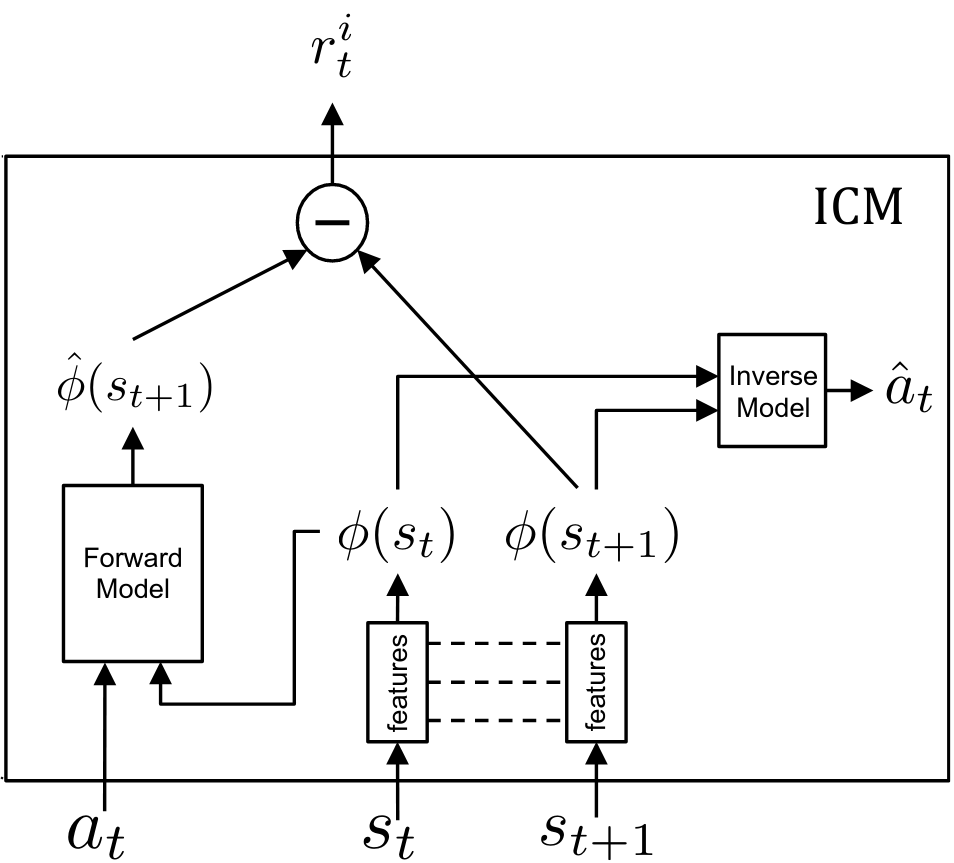
\includegraphics[width=0.6\textwidth]{figures/icm.png}
        \caption[The \gls{icm} by \citeauthor{pathak_curiosity-driven_2017-1}]{The \gls{icm} by \citeauthor{pathak_curiosity-driven_2017-1} where $r_t^i$ denotes the curiosity based intrinsic reward.\protect\footnotemark}
        \label{fig:icm}
    \end{figure}

    \footnotetext{\citep[3]{pathak_curiosity-driven_2017-1}}

    In summary, the encoding of the raw feature space using \gls{rf} showed that a curiosity based agent can be a very good competition to other state-of-the-art methods and are especially well-suited for simpler environments with less sophisticated visual observations.
    This is due to the fact that in these settings it is easier to preserve enough important information over the raw signal and thus be sufficient.
    A good example for this is the simulated environment of the Atari 2600 gaming console where \gls{rf} performed better in over 70\% when compared to an agent that chooses its actions arbitrarily.
    Although the performance of \gls{rf} is rather good as the features generalize badly across different environments.
    Here, the encoding with \gls{idf} performs better as it can transfer learned features from, e.g.\ one \textit{Mario Bros} level to another~\citep{burda_large-scale_2018-1}.
    Additionally, the \gls{idf}-curious agent was able to achieve a better score than a random agent in over 75\% of the Atari 2600 games and when compared to a \gls{rf}-curious agent, it performed better 55\% of the time, thus making \gls{idf} the preferred encoding.
    Concerning \gls{vae} methods for $\phi$, they perform either worse or the same as \gls{rf} or \gls{idf} and additionally were somewhat unstable.

    Unfortunately, all of these feature encodings are unable to deal with the white-noise problem which was mentioned in section~\ref{sec:problem-description}.

    Another selected approach is the paper "\usebibentry{kim_emi_2019}{title}" by \citeauthor{kim_emi_2019}
    With a similar action space as in the work by \citeauthor{pathak_curiosity-driven_2017-1}, they managed to improve significantly the agent's performance in several Atari 2600 games.
    However, this fell at the expenses of multiple additional layers of complexity.
    Instead of training a complex forward model that predicts the next encoded state, they transformed the complexity into a maximization problem of mutual information $I$ between $I([s,a];s')$ and $I([s,s'];a)$ and only used a simple linear model for $F$ to represent the space~\citep{aubret_survey_2019}.
    Concerning the problem with stochasticity, \citeauthor{kim_emi_2019} were able to tackle occurring white-noise by proposing an additional \textit{error model} which offloads non-linearity from the model $F$.
    By doing so, screen transitions, e.g.\ moving from one room to another in \textit{Montezuma's Revenge}, which are hard to predict and similar to white-noise, can be bypassed.


    \section{State Novelty}\label{sec:state-novelty}

    A further important approach to enable exploration by \gls{im} is the idea of state novelty where the agent earns intrinsic rewards when it enters states it has not visited before.
    This kind of idea can be formalized as a \textit{count-based} function which decreases the agent's intrinsic reward for entering a certain state depending on how often it had already visited this state before.
    Formally, the count-based function is denoted as the following:
    \begin{equation}
        R_{int}=\frac{1}{N(s_t)}
    \end{equation}
    where $N(s_t)$ stands for a counter which represents the agent's number of visits of the state $s_t$~\citep{aubret_survey_2019}.
    As one can imagine, this method is only efficient in discrete state spaces as in continuous ones the agent hardly visits states multiple times.

    A solution to this has been proposed by \citeauthor{bellemare_unifying_2016} which is based on density models that enable a \textit{pseudo-count}.
    By utilizing this method, the number of visits in a state as well as related neighbourhood states are combined to one counter which allows for better generalization.
    Therefore, the previously made notation is adapted to the following equation:
    \begin{equation}
        R_{int}=\frac{1}{\hat{N}(s_t)}
    \end{equation}
    where $\hat{N}(s_t)$ defines the pseudo-count which is denoted as follows:
    \begin{equation}
        \hat{N}(s_t)=\frac{p(s)(1-p'(s))}{p'(s)-p(s)}
    \end{equation}
    Here, $p(s)$ stands for a density model which calculates the probability of entering state $s$ and $p'(s)$ is the probability to visit state $s$ afterwards.
    The usage of the pseudo-count based on density models yield good results which enable exploration but add additional layers of complexity~\citep{aubret_survey_2019}.

    For the next method, \citeauthor{burda_exploration_2018} built upon their idea of using \gls{rf} but this time utilizing the encoding to combine it with a pseudo-count based approach that enables exploration through state novelty.
    However, they still somewhat made usage of prediction errors as they deployed a second \gls{nn} which solely fulfils the purpose of predicting the output of the random initialized one.
    The idea behind this is that the second \gls{nn} will produce a rather large error if the agent has never visited a specific state but over time gets more certainty about its predictions the more the agent has been in that state.
    By doing so, not only were they able to reduce the complexity of previous proposed methods such as the one which is based on density models but they also achieved one of the best scores in \textit{Montezuma's Revenge}~\citep{ecoffet_go-explore_2019}.

    One more selected state-novelty based approach is the one by \citeauthor{kim_curiosity-bottleneck_2019-1} who utilized the possibility of distilling recent states into a probability distribution.
    In their paper "\usebibentry{kim_curiosity-bottleneck_2019-1}{title}", they propose a method which produces a latent state space with a distribution of very large entropy that is based on their prior work of maximizing mutual information.
    Stating \citeauthor{aubret_survey_2019}:

    \begin{quote}
        "The intrinsic reward for a state is then the KL-divergence between a fixed diagonal Gaussian prior and the posterior of the distribution of latent variables.
        It results that, as long as the agent does not find any reward, it will look for rare states which have a distribution in the latent space that is different from the prior (common states fit the prior).
        When the agent finds the reward, the latent distribution will be different from the prior and the intrinsic reward will guide the agent towards interesting areas."

        \hfill~\cite[\p{12}]{aubret_survey_2019}
    \end{quote}

    Referring to section~\ref{sec:embeddingglsinto-theglsframework}, \citeauthor{kim_curiosity-bottleneck_2019-1} also made usage of \gls{em} by utilizing an extrinsic reward signal to tackle stochasticity which originates from white-noise.


    \section{Information Gain}\label{sec:information-gain}

    A final method to allow exploration is exploration via information gain.
    In this case, an intrinsic reward is credited depending on the agent's ability to reduce uncertainty of the dynamics of its environment.
    By using information-gain based methods, the agent can be led to states it is rather uncertain about while at the same time being able to predict environment transitions.
    Therefore, the agent is unaffected of the white-noise problem based on stochasticity or state transitions~\citep{aubret_survey_2019}.
    Furthermore, under the usage of the parameter set $\theta$ which is used in a parametric model and the function $U$ which defines uncertainty, the information gain can be formalized as follows:

    \begin{equation}
        R_{int}=U_{t+k}(\theta) - U_t(\theta)
    \end{equation}

    A well-suited example to introduce information-gain based approaches is "\usebibentry{pathak_self-supervised_2019}{title}" by \citeauthor{pathak_self-supervised_2019}
    Here, the authors use multiple \glspl{nn} or rather forward models to predict the next state $s_{t+1}$ based on a state-action tuple.
    Further, the different predictions of the subsequent state $s_{t+1}$ are composed and their variance acts as the intrinsic reward.
    Depending on the number of trained networks, the more forward models are learned, the better the performance of the agent will be as the models' predictions will converge to the expected observation of state $s_{t+1}$.
    Moreover, for illustration purposes, the algorithm is visualized in Figure~\ref{fig:ensemble_dissagreement}.

    By utilizing the variance of the predictions, the agent's desired behaviour is depicted as a high variance that solely occurs if the models are not trained yet which forces the agent to explore.
    Concerning stochasticity, this problem is also solved by the variance since the irritating white-noise becomes irrelevant as the average of all predictions converges truthfully.
    Hence, this approach yields good performance when compared to other state-of-the-art methods but is very computationally expensive due to the necessity of training multiple forward models.

    \begin{figure}[h]
        \centering
        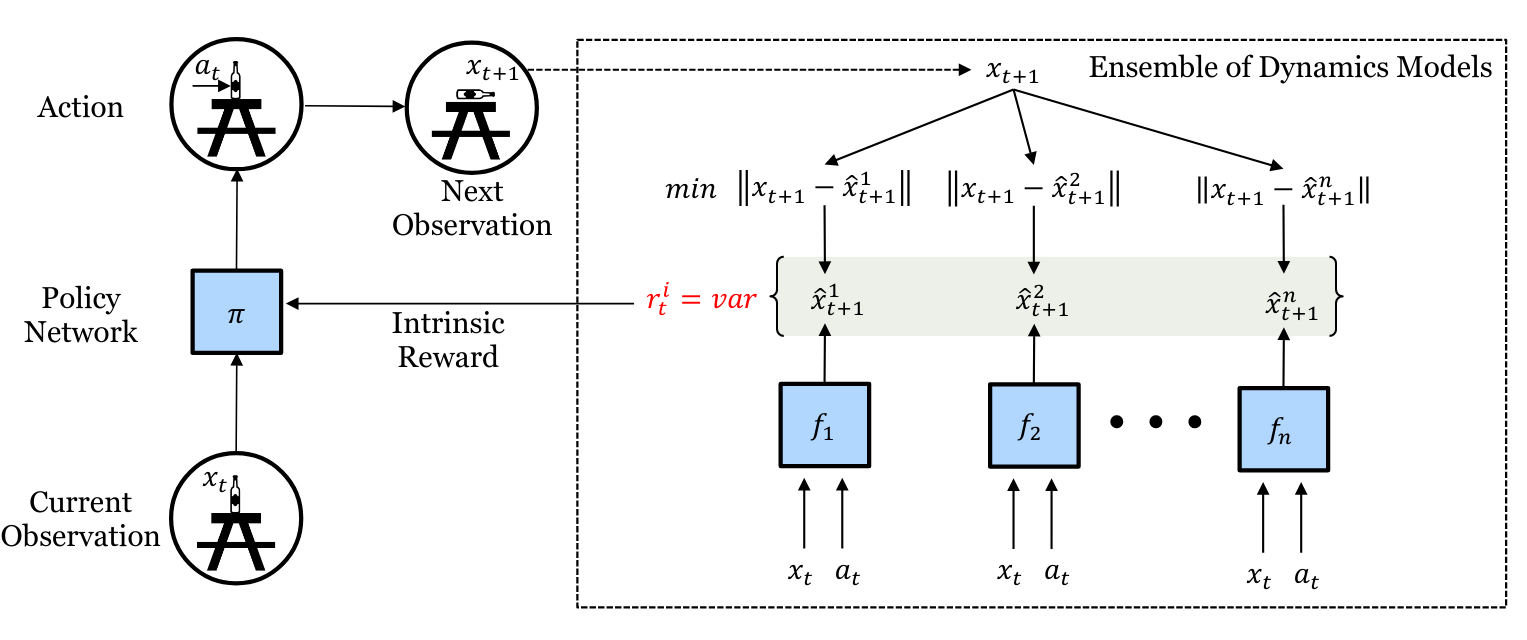
\includegraphics[width=\textwidth]{figures/ensemble_dissagreement.png}
        \caption[A visualisation of the algorithm introduced in "\usebibentry{pathak_self-supervised_2019}{title}"]{A visualisation of the algorithm introduced in "\usebibentry{pathak_self-supervised_2019}{title}" where the current observation is denoted as $x_t$ and $r_t^i$ stands for the intrinsic reward.\protect\footnotemark}
        \label{fig:ensemble_dissagreement}
    \end{figure}

    \section{Current State of the Art Method}

    The current record on \textit{Montezuma's Revenge} is held by \citeauthor{ecoffet_go-explore_2019} who were able to drastically improve the state of the art with a four times higher score than previously introduced methods.
    Despite the fact that \gls{im} algorithms are usually the best performing solutions to encourage exploration in sparse environments, by the introduction of their paper "\usebibentry{ecoffet_go-explore_2019}{title}", the authors presented a promising solution which however is not based on \gls{im}.
    Surprisingly, their exploration method is based on an agent that selects actions randomly, an approach which on its own would usually not perform well.
    However, they added a significant prior step to exploration as they teach the agent to re-enter a previously visited promising position before it starts exploring again.
    This step solves a fundamental issue of intrinsically motivated exploration which can be observed in Figure~\ref{fig:exploration_problem}.
    Although \gls{im} is normally the standard approach to environments with sparse rewards, they all have one fundamental problem in common where the agent fails to re-enter already visited states as the path which leads to these states is not interesting anymore and thus hinders the agent to further discover its environment.

    \begin{figure}[h]
        \centering
        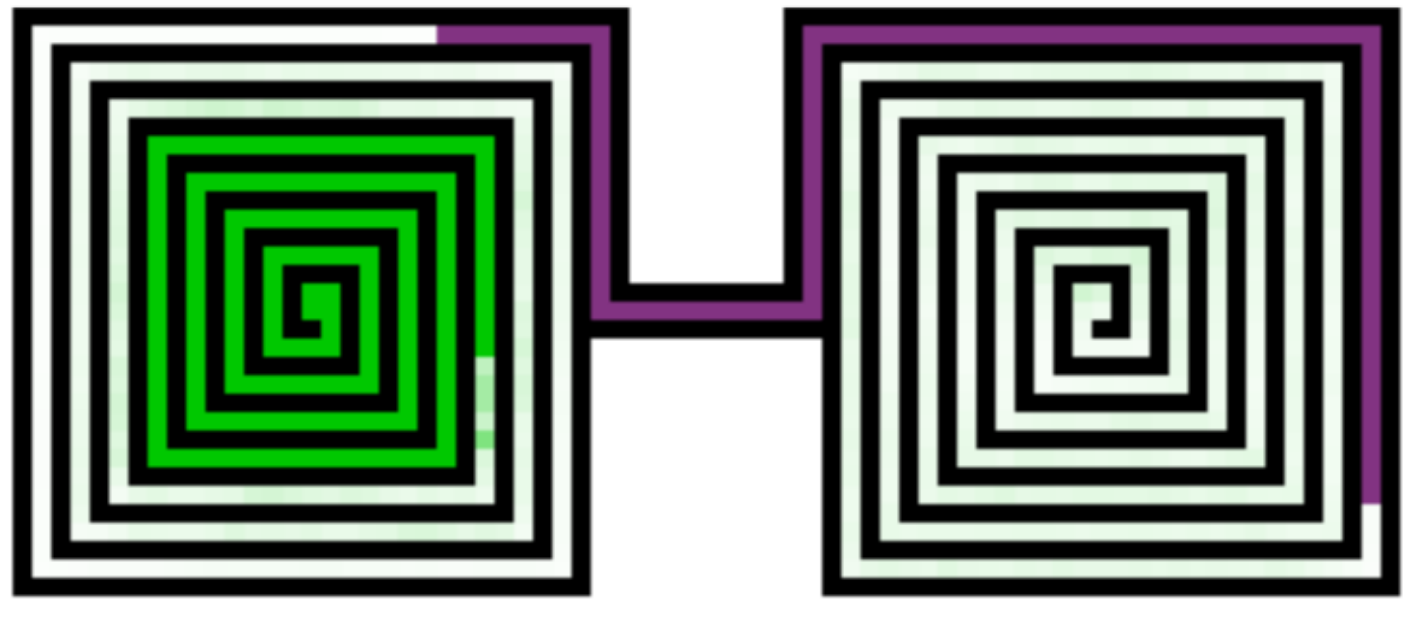
\includegraphics[width=0.75\textwidth]{figures/exploration_problem.png}
        \caption[An illustration of intrinsically motivated exploration methods where an agent is unable to rediscover promising areas]{An illustration of intrinsically motivated exploration methods where an agent is unable to rediscover promising areas\protect\footnotemark}
        \label{fig:exploration_problem}
    \end{figure}

    \footnotetext{\citep[\p{3}]{ecoffet_go-explore_2019}}

    In Figure~\ref{fig:exploration_problem}, this problem is illustrated where the white path denotes already discovered parts of an agent's environment, the green one stands for intrinsic rewards it has yet to obtain, and the purple area marks the path it has explored in the current episode.
    This example shows the problem of an agent who is uninterested in visiting known states again and thus unable to ever discover the green intrinsically rewarding area.

    According to the authors, their exploration algorithm is structured as follows:


    \begin{quote}
        "It exploits the following principles: (1) remember states that have
        previously been visited, (2) first return to a promising state (without exploration),
        then explore from it, and (3) solve simulated environments through exploiting any
        available means (including by introducing determinism), then robustify (create a
        policy that can reliably perform the solution) via imitation learning."

        \hfill~\cite[\p{1}]{ecoffet_go-explore_2019}
    \end{quote}

    A graphical illustration of this algorithm can be inspected in Figure~\ref{fig:go_explore} where states are encoded in so-called cells which are low-resolution, grey-scale images.

    With this algorithm, the trained agent was able to achieve superhuman performance and thus surpass human players in the game of \textit{Montezuma's Revenge}.
    Furthermore, in another difficult exploration game called \textit{Pitfall}, their algorithm was the first one which managed a score above zero.
    Lastly, another achievement worth mentioning is that it outperformed state-of-the-art solutions of imitation learning where an agent is trained on recorded man-made gameplay due to the fact that their approach can cheaply create such demonstrations on its own.
    For all these reasons, \textit{Go-Explore} is a very promising direction for further research, especially focusing on how to combine existing methods with this novel idea.

    \newpage

    \begin{figure}[h]
        \centering
        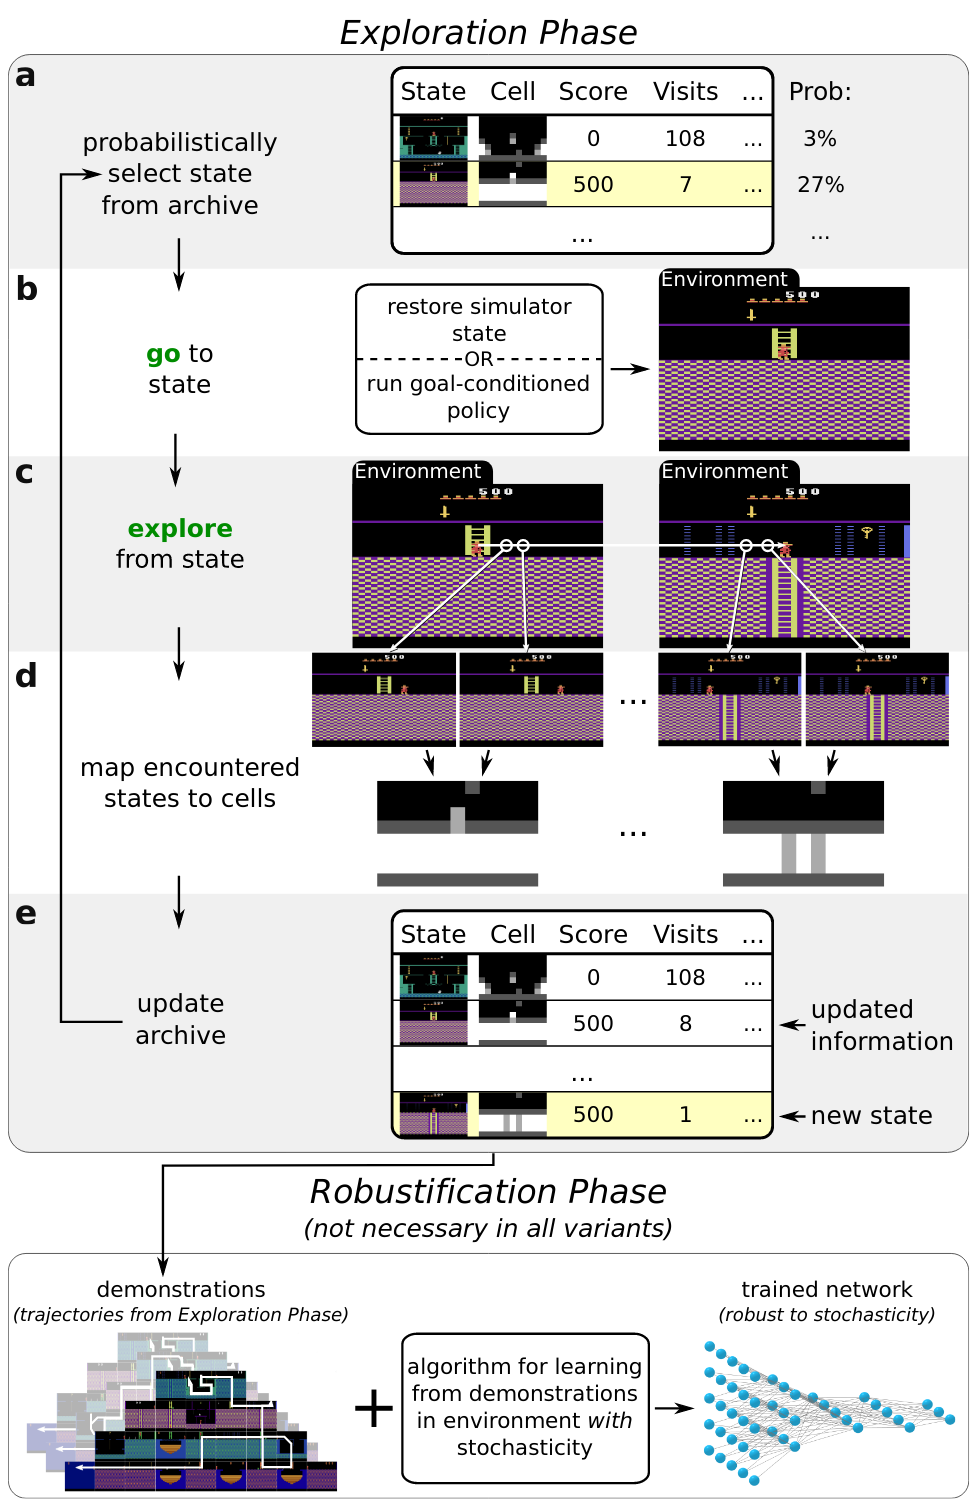
\includegraphics[width=0.70\textwidth]{figures/go_explore.png}
        \caption[The simple, yet astonishingly good performing algorithm "Go-Explore"]{The simple, yet astonishingly good performing algorithm "Go-Explore" by \citeauthor{ecoffet_go-explore_2019} which is currently the best performing approach to \textit{Montezuma's Revenge}, directly follow by "Random Network Distillation" from the authors \citeauthor{burda_exploration_2018} \protect\footnotemark}

        \label{fig:go_explore}
    \end{figure}

    \footnotetext{\citep[\p{3}]{ecoffet_first_2020}}

    \glsresetall


    \chapter{Implementation}\label{ch:implementation}
    \citep{burda_large-scale_2018-1}
    \citep{pathak_curiosity-driven_2017-1}


    \section{Proximal Policy Optimization}
    Hyperparameter


    \section{Intrinsic Curiosity Module}
    \citep{pathak_curiosity-driven_2017-1}


    \section{Hyper-Parameter Tuning}
    %TODO Gridsearch


    \section{Noisy-TV Problem}
    \citep{schmidhuber_formal_2010}

    \glsresetall


    \chapter{Evalutation}
%TODO 9. Benchmarking Deep RL
    \citep{francois-lavet_introduction_2018}

    \glsresetall


    \chapter{Results}
    For a performance comparison, we orientate ourselves on \textit{Table 3}, created by~\cite{aubret_survey_2019}. This table summarizes state of the art methods on exploration strategies with IM and points out the mean score of theses methods on \textit{Montezuma's revenge}.

    \begin{figure}[h]
        \begin{center}
            \begin{subfigure}{.3\textwidth}
                \centering
                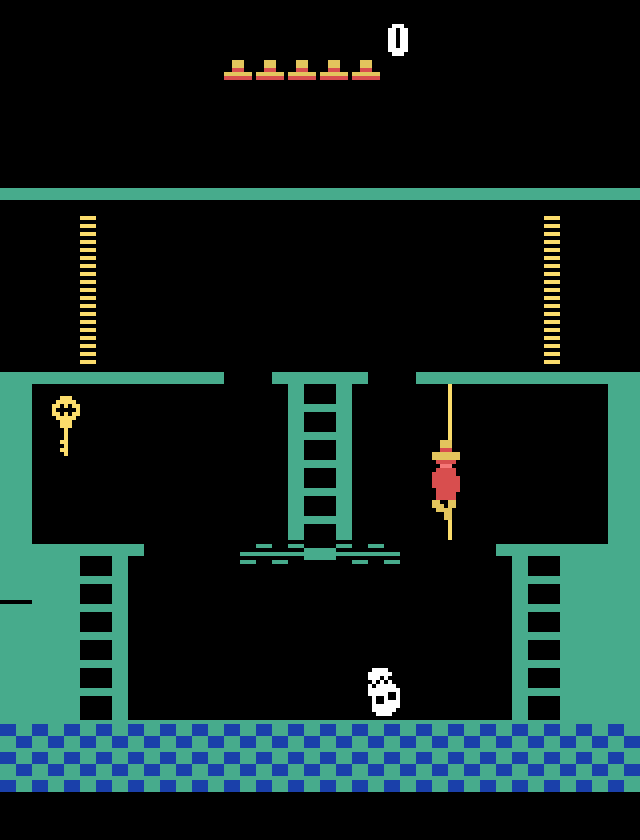
\includegraphics[width=.8\linewidth]{figures/montezumarevenge.png}
                \caption{Montezuma's Revenge}
                \label{fig:mz}
            \end{subfigure}%
            \begin{subfigure}{.3\textwidth}
                \centering
                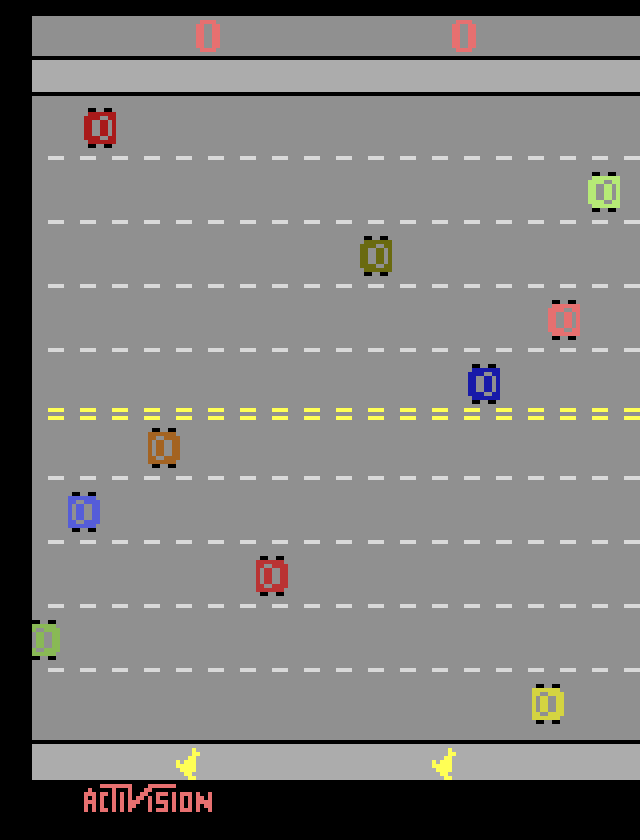
\includegraphics[width=.8\linewidth]{figures/freeway.png}
                \caption{Freeway}
                \label{fig:fway}
            \end{subfigure}
            \begin{subfigure}{.3\textwidth}
                \centering
                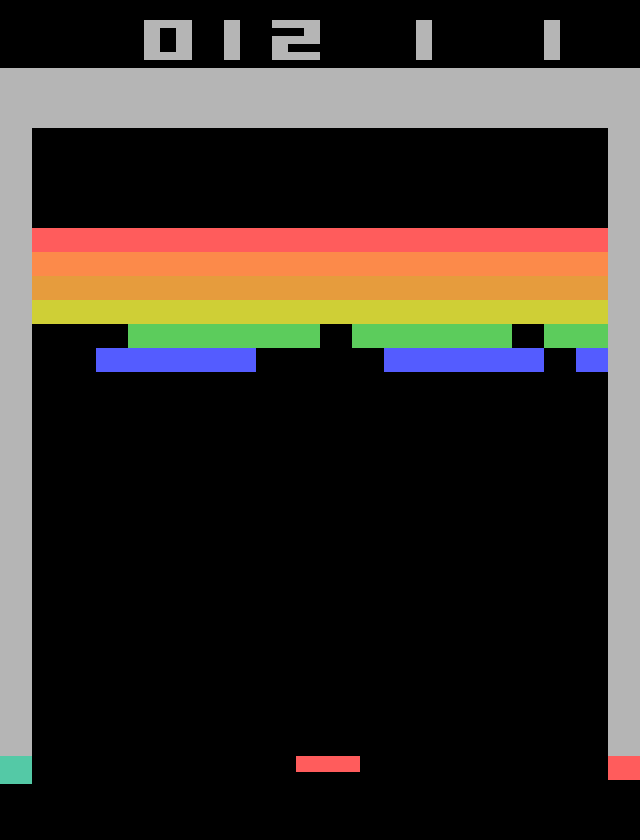
\includegraphics[width=.8\linewidth]{figures/breakout.png}
                \caption{Breakout}
                \label{fig:break}
            \end{subfigure} \caption{The gameplay of three selected Atari 2600 games}
            \label{fig:games}
        \end{center}
    \end{figure}


    \section{Montezuma's Revenge}


    \section{Freeway}


    \section{Breakout}


    \begin{figure}[h]
        \centering
        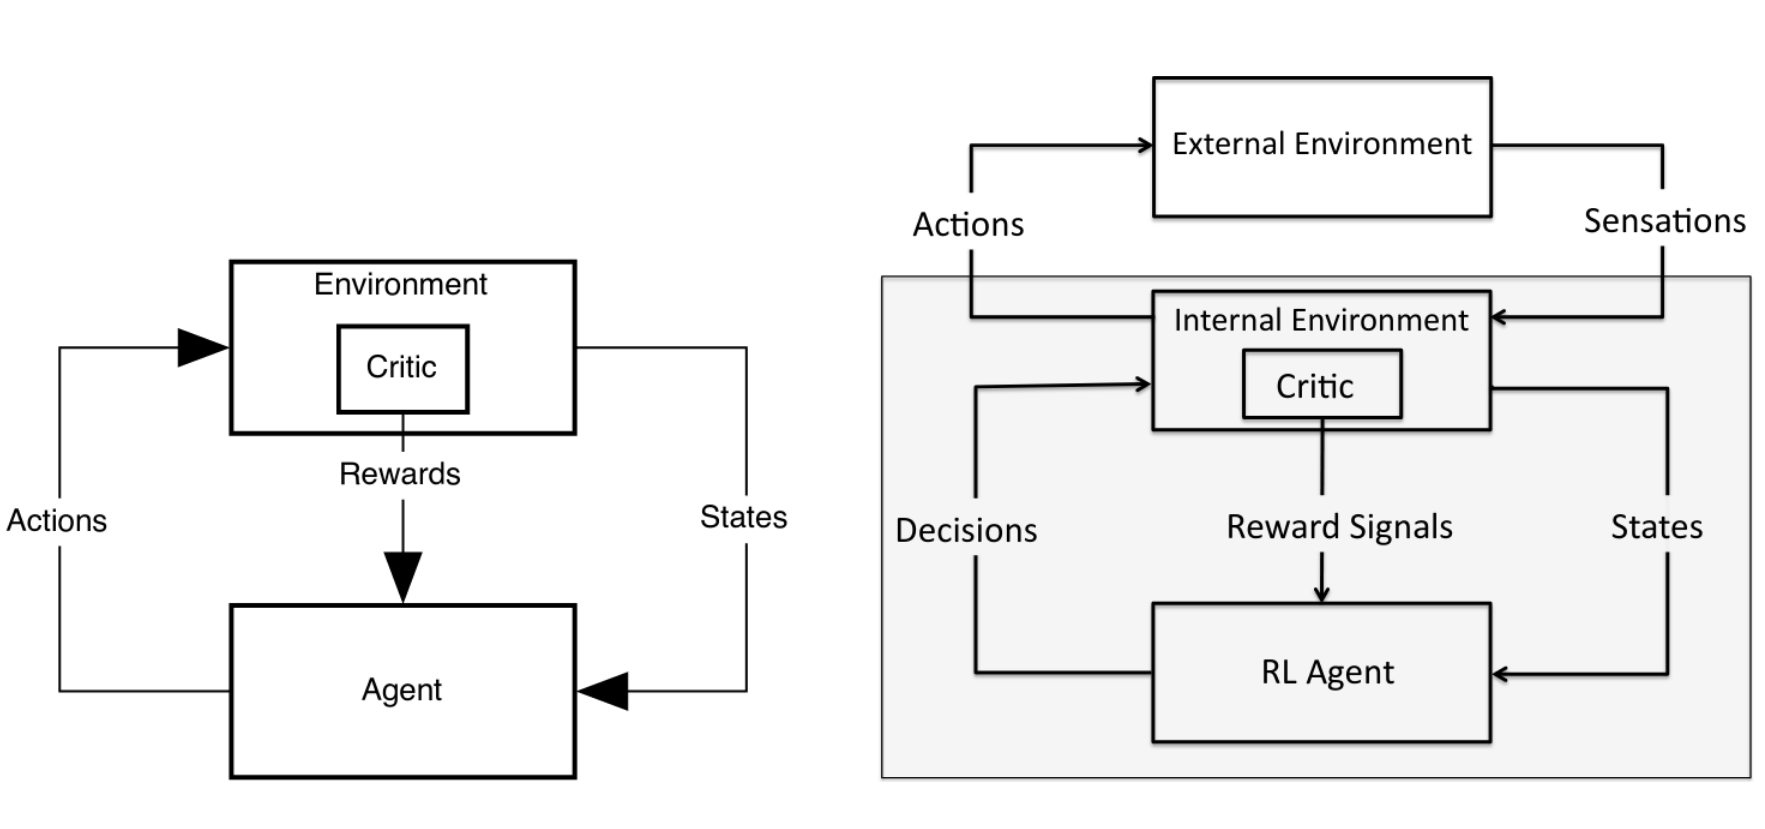
\includegraphics[width=\textwidth]{figures/adapted_rl_framework.png}
        \begin{scriptsize}
            \vspace{0.2cm}
            \begin{tabular}{|lcc|}
                \hline
                &                                             &                                                 \\
                \textbf{Extrinsic Only:}           &                                             & \colorindicator{tab:green}{INT=0.00, EXT=1.00}  \\
                \textbf{Random Features:}          & \colorindicator{tab:red}{INT=1.0, EXT=0.0}  & \colorindicator{tab:orange}{INT=0.43, EXT=0.57} \\
                \textbf{Inverse Dynamic Features:} & \colorindicator{tab:blue}{INT=1.0, EXT=0.0} & \colorindicator{tab:purple}{INT=0.43, EXT=0.57} \\
                &                                             &                                                 \\
                \hline
            \end{tabular}

        \end{scriptsize}
        \def\arraystretch{1.3}
        \begin{scriptsize}
            \begin{tabular}{|ccc|}
                \hline
                \textbf{Random Features}                                                                   & \textbf{Extrinsic Only}                      & \textbf{Inverse Dynamic Features}                                                           \\
                \colorindicator{tab:red}{INT=1.0, EXT=0.0}|\colorindicator{tab:orange}{INT=0.43, EXT=0.57} & \colorindicator{tab:green}{INT=0.0, EXT=1.0} & \colorindicator{tab:blue}{INT=1.0, EXT=0.0}|\colorindicator{tab:purple}{INT=0.43, EXT=0.57} \\
                \hline
            \end{tabular}

        \end{scriptsize} \caption{This is a test for the caption}


    \end{figure}

    \glsresetall


    \chapter{Conclusion and Further Work}

    \backmatter
% Use an optional list of figures.
    \listoffigures % Starred version, i.e., \listoffigures*, removes the toc entry.

% Use an optional list of tables.
    \cleardoublepage % Start list of tables on the next empty right hand page.
    \listoftables % Starred version, i.e., \listoftables*, removes the toc entry.

% Use an optional list of alogrithms.
    \listofalgorithms
    \addcontentsline{toc}{chapter}{List of Algorithms}

% Add an index.
    \printindex

% Add a glossary.
    \printglossaries

% Add a bibliography.
    \bibliographystyle{abbrvnat}
    \bibliography{core}

    \bibliographystyleOnline{abbrvnat}
    \bibliographyOnline{online}
\end{document}
